\documentclass{patmorin}
\usepackage[utf8]{inputenc}
\usepackage{amsmath,amsfonts,amssymb,amsthm,graphicx,graphics}
%\setcounter{tocdepth}{3}
\usepackage{graphicx}

%\usepackage{algorithmic}
%\usepackage{algorithm}
\usepackage{hyperref}
\usepackage[dvipsnames]{xcolor}
\definecolor{linkblue}{named}{Blue}
\hypersetup{colorlinks=true, linkcolor=linkblue,  anchorcolor=linkblue,
citecolor=linkblue, filecolor=linkblue, menucolor=linkblue,
urlcolor=linkblue} 

\setlength{\parskip}{2ex}

%\usepackage{comment}
%\usepackage{url}
%\usepackage{xspace} 
%\usepackage{lineno}
%\graphicspath{{img/}} % No need to write this for every figure
%\linenumbers


%\usepackage{geometry}

\newcommand{\etal}{\emph{et al}}

\newtheorem{theorem}{Theorem}[section]
\newtheorem{corollary}[theorem]{Corollary}
\newtheorem{lemma}[theorem]{Lemma}
\newtheorem{proposition}[theorem]{Proposition}
\newtheorem{observation}[theorem]{Observation}
\newtheorem{problem}[theorem]{Problem}
\newtheorem{definition}[theorem]{Definition}
\newtheorem{conjecture}[theorem]{Conjecture}
\newtheorem{question}[theorem]{Question}

\DeclareMathOperator{\rank}{rank}

\newcommand{\R}{\mathbb{R}}


%%
%% Here you may place your macros using \newcommand{}{}
%%
  
\newcommand{\red}[1]{{\color{red} #1}}
  
\newcommand{\ch}[1]{\ensuremath{\textsc{ch}(#1)}}

\title{\MakeUppercase{Compatible Connectivity-Augmentation \newline of Disconnected Graphs}}

%\author{Second Bellairs Workshop on Geometry and Graphs}
\author{Greg Aloupis \and Luis Barba \and Paz Carmi \and Fabrizio Frati
        \and Vida Dujmović \and Pat Morin}



\begin{document}

\begin{titlepage}

\maketitle
\begin{abstract}
\setlength{\baselineskip}{16.8pt}
We consider the following \emph{compatible connectivity-augmentation
problem}: We are given a planar graph,
$\mathcal{G}$, that has $r>1$ connected components, and $k$ isomorphic planar drawings, $G_1,\ldots,G_k$, of
$\mathcal{G}$. We wish to add vertices and edges to $\mathcal{G}$ to make
it connected and in such a way that these vertices and edges can be added to
the drawings $G_1,\ldots,G_k$ while preserving planarity.  We show that
adding $\Theta(nr^{1-1/k})$ edges and vertices to $\mathcal{G}$ is always
sufficient and sometimes necessary to achieve this goal.  
\end{abstract}

\end{titlepage}

%A category including the fourth, optional field follows..

\section{Introduction}


We consider the following problem, which will be more carefully formalized
below.  We are given several different planar straight-line drawings
of the same graph, $\mathcal G$, which is not connected.
We wish to make $\mathcal G$ connected by adding vertices and edges in
such a way that these vertices and edges can also be added to the planar
straight-line drawings of $\mathcal G$ while preserving the planarity of
the drawings.  The objective is to do this while minimizing the number
of edges and vertices added.  As the example in Figure~\ref{fig:bad-example} shows, it is not always possible to just add edges to $\mathcal G$; sometimes additional vertices are necessary.

\begin{figure}
  \centering{
    \begin{tabular}{c@{\hspace{2cm}}c}
      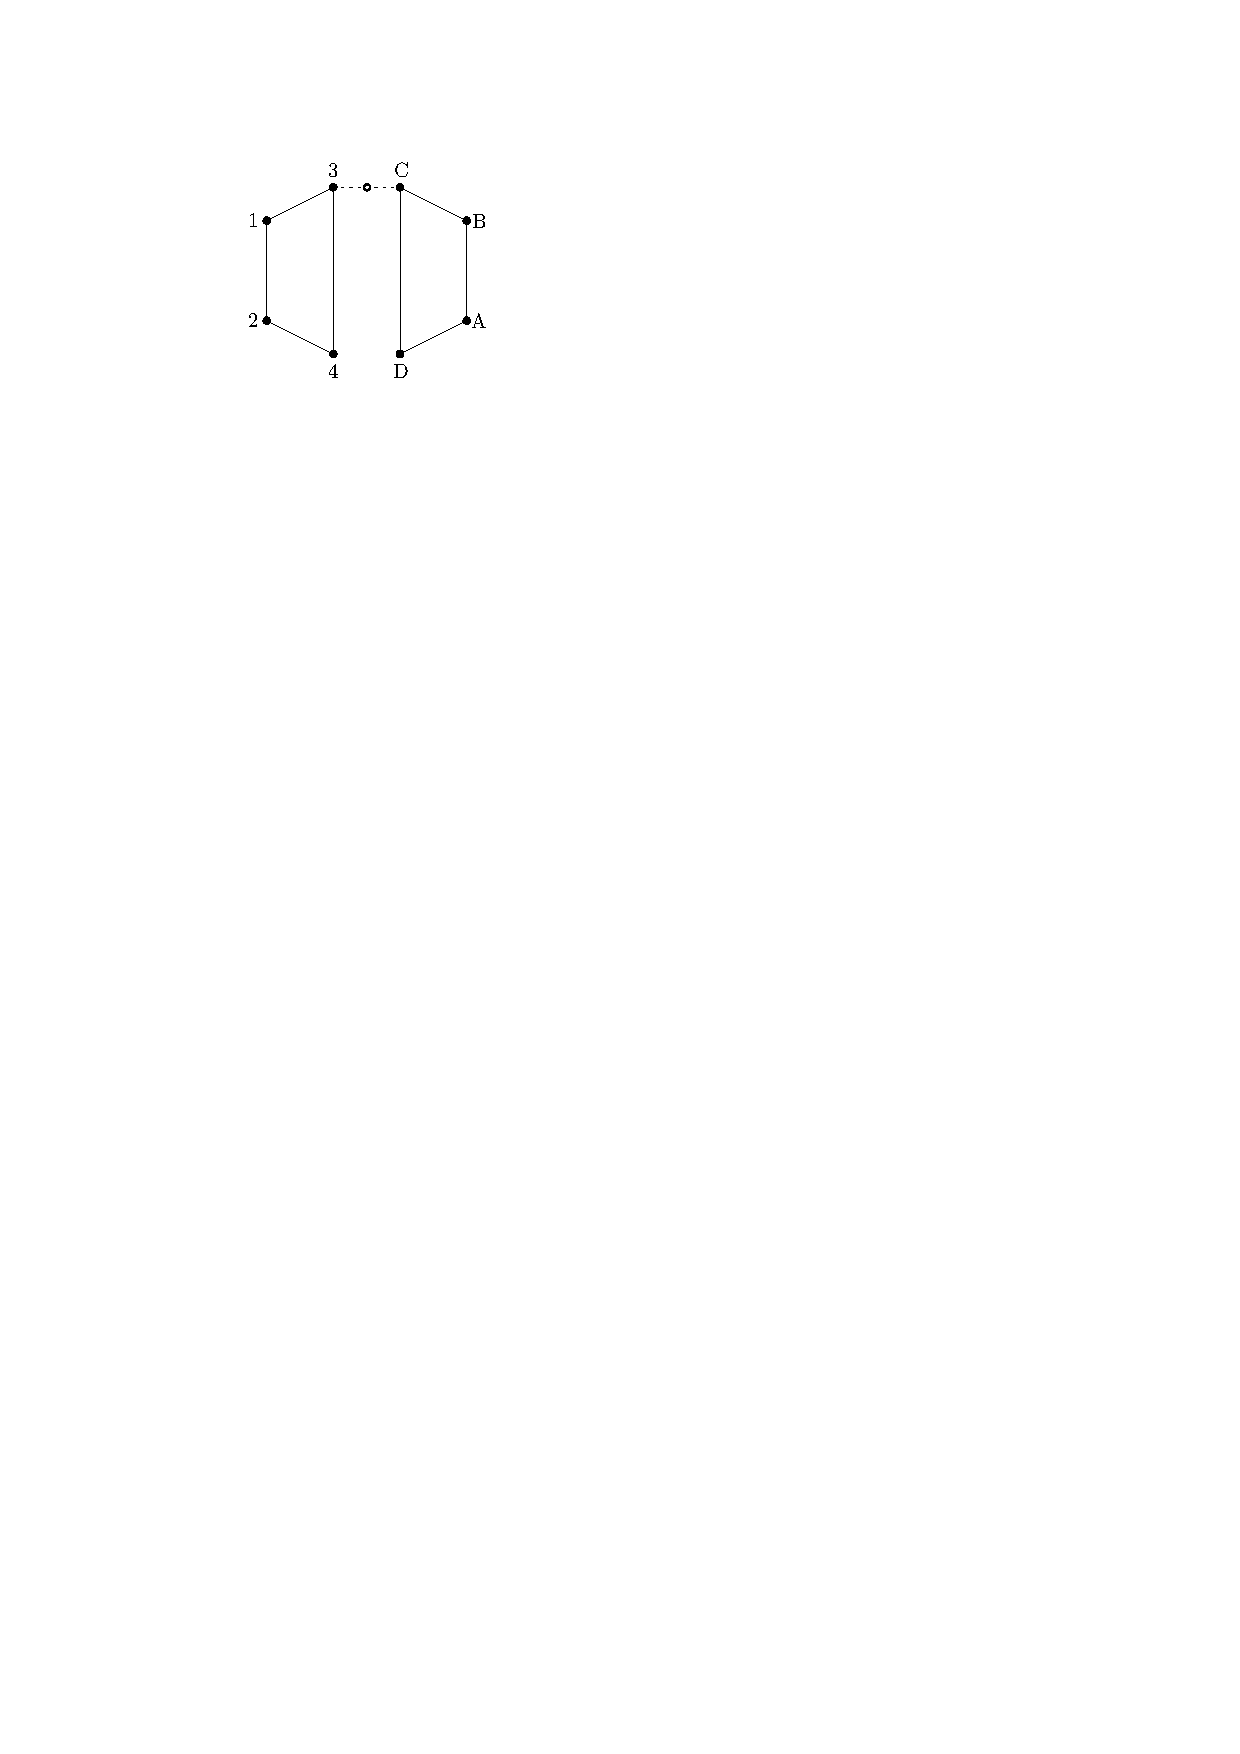
\includegraphics{img/bad-example-1} & 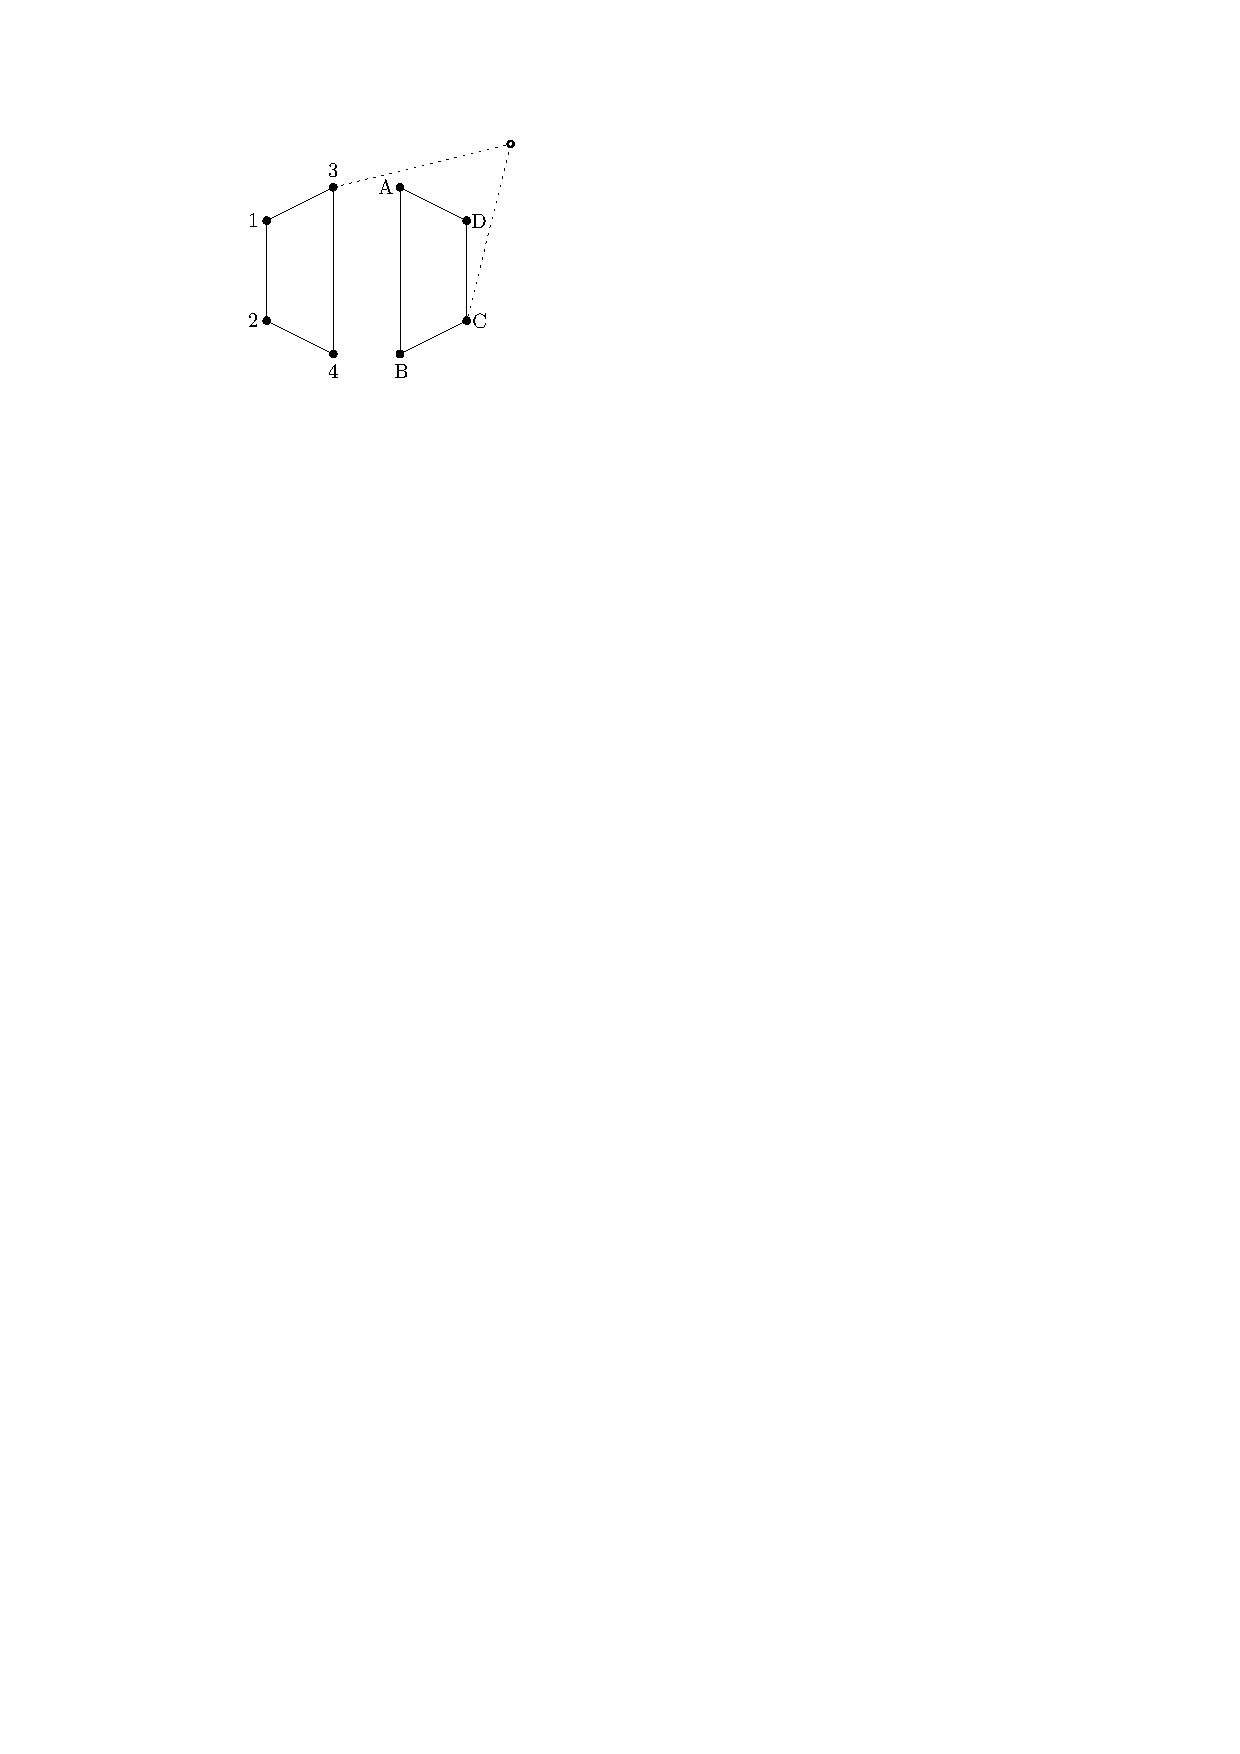
\includegraphics{img/bad-example-2}
    \end{tabular}
  }
  \caption{Two drawings of the same graph, $\mathcal{G}$, where making $\mathcal{G}$ connected requires the addition both of edges and vertices. In this case, $\mathcal G$ is made connected by adding the hollow vertex and two dashed edges.}
  \label{fig:bad-example}
\end{figure}

The motivation for studying this problem comes from the problem of morphing
planar graphs, which has many applications \cite{erten.kobourov.ea:intersection,friedrich.eades:graph,gotsman.surazhsky:guaranteed,surazhsky.gotsman:controllable,surazhsky.gotsman:intrinsic} including
computer animation.  Imagine an
animator who wishes to animate a scene in which a character's expression
goes from neutral, to surprised, to happy. The animator can draw these
three faces, but does not want to hand-draw the 30--60 frames required
to animate the change of expression.  The strokes used to draw the
character's features can be converted into paths and these can be merged
into components corresponding to the character's eyes, nose, mouth and
so on.  A correspondence between the same elements in different pictures
is also given.\footnote{In many cases, the correspondence is a byproduct
of the creation process. For example, in Figure~\ref{fig:faces}, the second
two faces were obtained by copying and then editing the first one.}  Thus,
the input is three isomorphic drawings of the same planar graph.

\begin{figure}
  \centering{ 
  \begin{tabular}{c@{\hspace{1cm}}c@{\hspace{1cm}}c}
    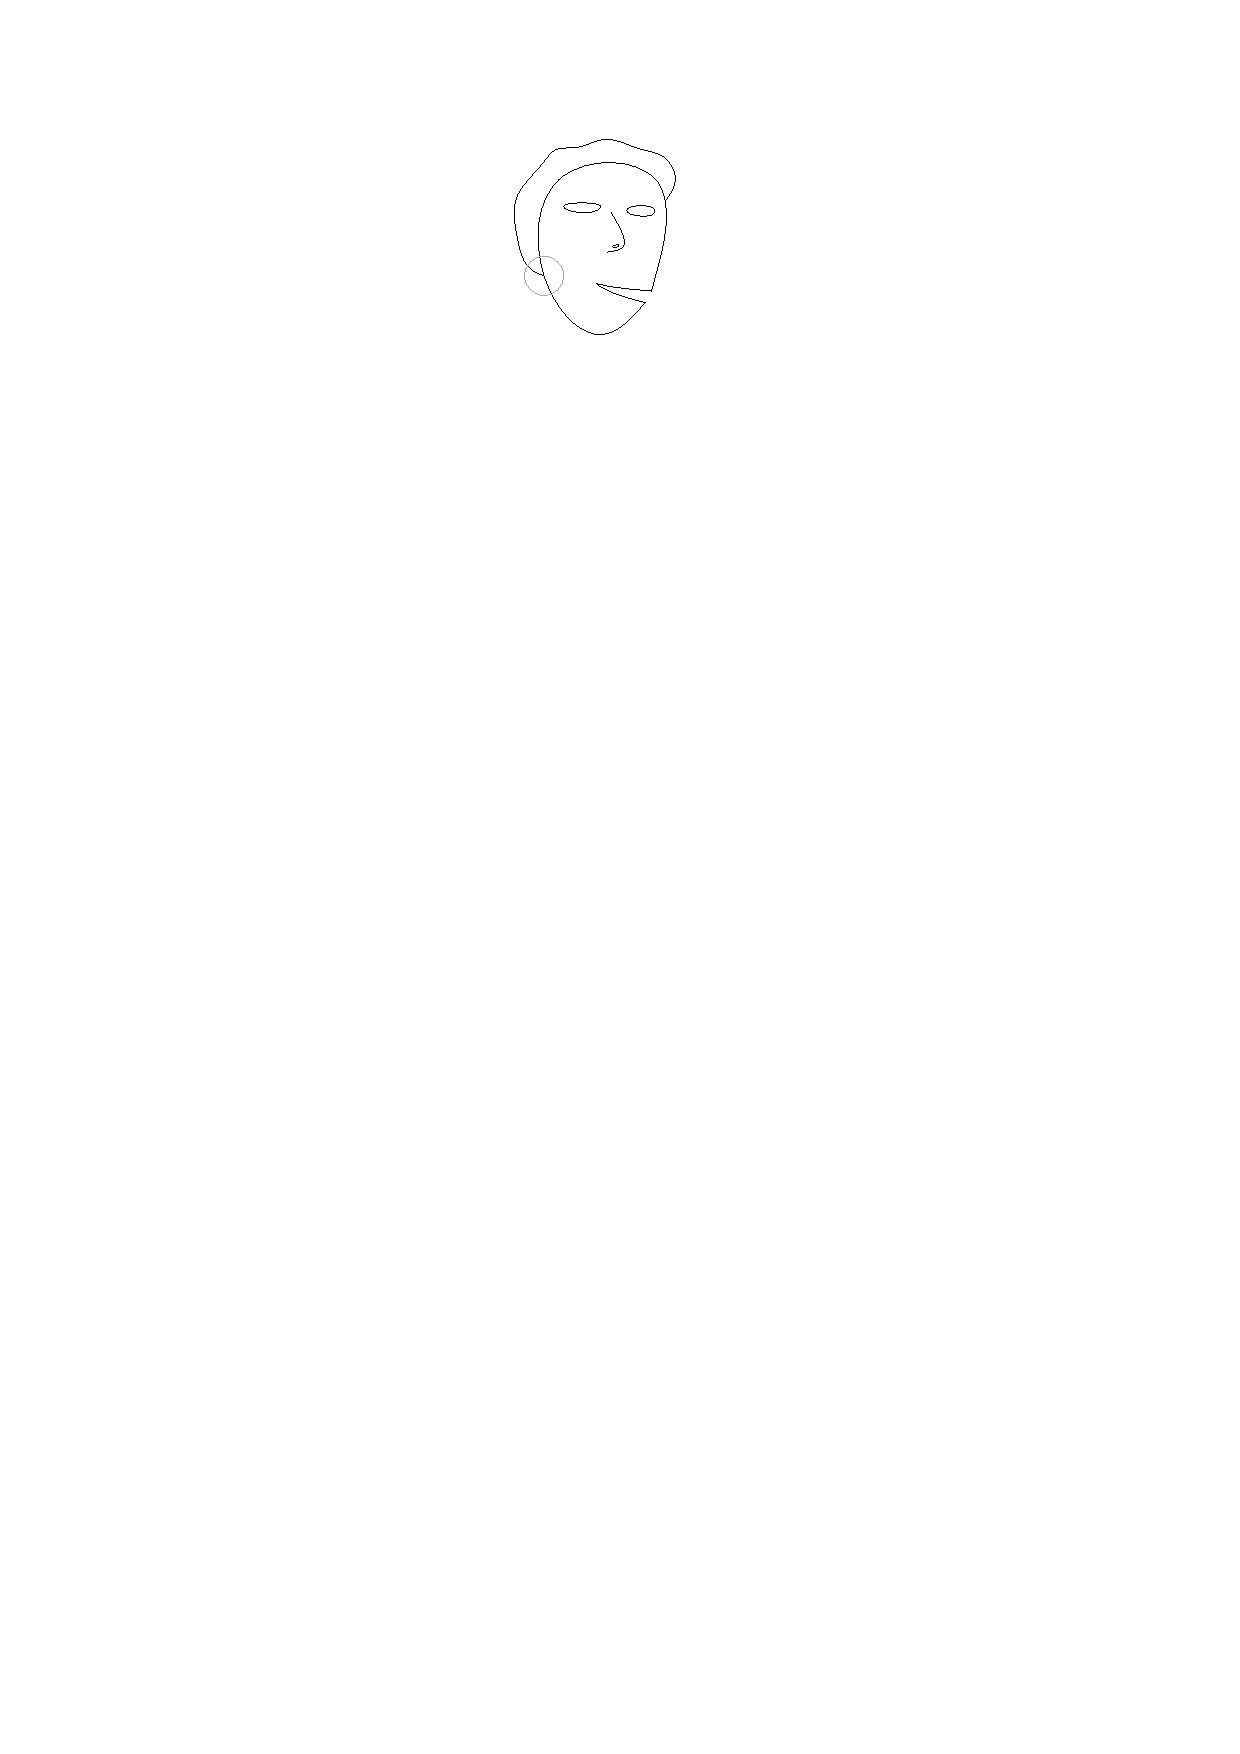
\includegraphics{img/faces-1} &
    
\includegraphics{img/faces-2} &
    
\includegraphics{img/faces-3} \\
    & 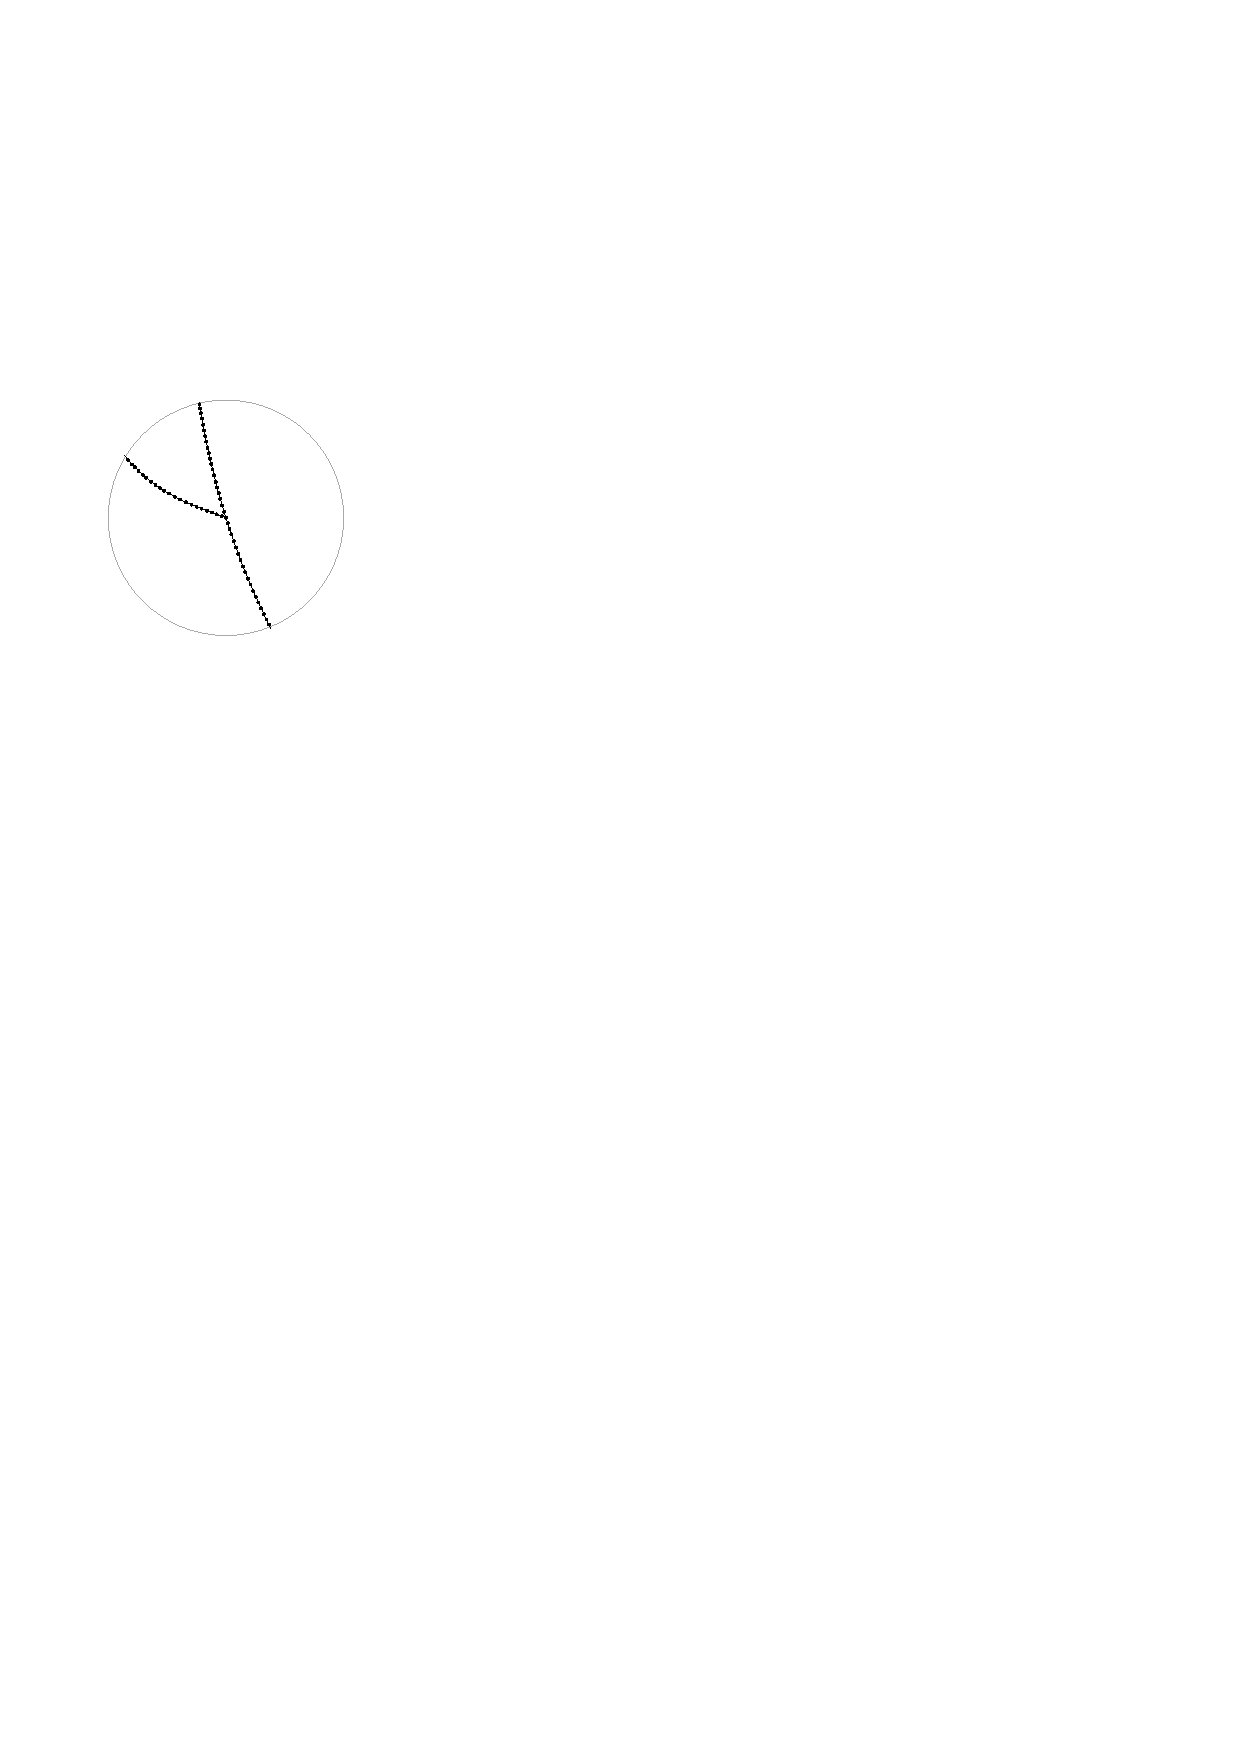
\includegraphics{img/face-zoom} &
  \end{tabular}}
  \caption{Computer-assisted animation frequently involves morphing between
   a sequence of drawings of the same planar graph.  Zooming in on a section
   of the image reveals that the artist's strokes are approximated by polygonal
   paths}
  \label{fig:faces}
\end{figure}

In this setting, animating the face becomes a problem of \emph{morphing}
(i.e., continuously deforming) one drawing of a planar graph into
another drawing of the same planar graph while maintaining planarity
of the drawing throughout the deformation. This morphing problem
has been studied since 1944, when Cairns \cite{cairns:deformations}
showed such a transformation always exists between any two drawings
of the same graph.  Since then, a sequence of results has shown
that such transformations can be done efficiently, so that the
motion can be described concisely \cite{thomassen:deformations,
grunbaum.shephard:geometry,alamdari.angelini.ea:morphing,
angelini.dalozzo.ea:morphing}.  The most recent such result
\cite{angelini.dalozzo.ea:morphing} shows that any planar drawing of
an $n$-vertex connected planar graph can be morphed into any isomorphic
drawing using a sequence of $O(n)$ \emph{linear
morphs}, in which vertices move along linear trajectories at constant
speed.

These morphing algorithms require that the input graph, $\mathcal{G}$,
be connected. In many applications of morphing (for example in
Figure~\ref{fig:faces}) the input graph is not connected. Before these
morphing algorithms can be used, $\mathcal{G}$ must be augmented into a
connected graph, $\mathcal H$, but this augmentation must be compatible
with the drawings of $\mathcal{G}$.  At the same time, the complexity
of the morph produced by a morphing algorithm depends on the number
of vertices of $\mathcal H$.  Therefore, we want to find an augmentation
with the fewest number of vertices.

This motivates the elegant theoretical question studied in the current paper:  How can we add
vertices and edges to $\mathcal{G}$ to obtain a supergraph $\mathcal
H\supset \mathcal G$ that is connected and such that the vertices and
edges of $\mathcal{H}$ can also be added to the drawings of $\mathcal{G}$
while maintaining the planarity of each drawing?  In this paper,
we obtain a tight bound for the extremal question: In the worst case
(over all $n$ vertex planar graphs, $\mathcal G$, and over all sets of
$k$ planar drawings of $\mathcal{G}$), how many edges have to be added
to $\mathcal{G}$ to obtain connectivity while preserving planarity of
the drawings?


\subsection{Formal Problem Statement and Main Result}

Formally, a \emph{drawing} of a graph $\mathcal{G}=(V,E)$
is a one-to-one function $\varphi\colon V\to\R^2$.  A drawing
is \emph{planar} if, for every pair of edges $uw$ and $xy$ in $E$,
the open line segment with endpoints $\varphi(u)$ and $\varphi(w)$ is
disjoint from the open line segment with endpoints $\varphi(x)$
and $\varphi(y)$.  Two planar drawings, $\varphi_1$ and $\varphi_2$,
of $\mathcal{G}$ are \emph{isomorphic} if there exists a continuous family
of planar drawings $\{\varphi^{(t)} \colon 0\le t\le 1\}$ of $\mathcal{G}$
such that $\varphi^{(0)}=\varphi_1$ and $\varphi^{(1)}=\varphi_2$.

Throughout this paper we will be slightly less formal to avoid repeatedly
referencing drawing functions like $\varphi$, $\varphi_1$ and $\varphi_2$.
Instead, we will talk about a graph $\mathcal{G}$ and $k$ isomorphic
geometric graphs $G_1,\ldots,G_k$.  This should be understood to mean that
each $G_i$ is the geometric graph given by the drawing of $\mathcal{G}$
with some function $\varphi_i$ and that $\varphi_1,\ldots,\varphi_k$ are
pairwise isomorphic.  When necessary, we may talk about the vertex $v$
in $G_i$ where $v$ is actually a vertex of $\mathcal{G}$; this should
be taken to mean the vertex $\varphi_i(v)$ in $G_i$.

With these conventions, we are ready to state our main result.  Given $k$
geometric planar isomorphic embeddings $G_1, \ldots, G_k$ of $\mathcal
G$, a \emph{compatible augmentation}, $\mathcal H$, of $\mathcal G$ is
a supergraph of $\mathcal G$ such that (1) $\mathcal H$ is connected,
and (2) there exist geometric planar isomorphic embeddings, $H_1,
\ldots, H_k$, of $\mathcal H$ such that $H_i\supset G_i$ for every
$i\in\{1,\ldots,k\}$.  In this paper, we show that, if $\mathcal{G}$ has
$n$ vertices and $r$ connected components, then there always exists a
compatible augmentation of size $O(nr^{1-1/k})$ and that this bound is
tight; there exists a graph $\mathcal G$ with $r$ components and having
embeddings $G_1,\ldots,G_k$ for which any compatible augmentation has
size $\Omega(nr^{1-1/k})$.

\subsection{Related Work}

To the best of our knowledge, there is very little work on
compatible connectivity-augmentation of planar graphs, though
there is work on isomorphic triangulations of polygons.  Refer to
Figure~\ref{fig:compatible-triangs}.  In this setting, the graph
$\mathcal{G}$ is a cycle and one has two non-crossing drawings, $P$
and $Q$, of $\mathcal G$. The goal is to augment $\mathcal G$ (and the
two drawings $P$ and $Q$) so that $\mathcal G$ becomes a near-triangulation,
and $P$ and $Q$ become (geometric) triangulations of the interiors
of the polygons whose boundaries are $P$ and $Q$.  Aronov \etal\
\cite{aronov.seidel.ea:compatible} showed that this can always
be accomplished with the addition of $O(n^2)$ vertices and that
$\Omega(n^2)$ vertices are sometimes necessary.  Kranakis and Urrutia
\cite{kranakis.urrutia:isomorphic} showed that this result can be made
sensitive to the number of reflex vertices of $P$ and $Q$, so that the
number of triangles required is $O(n+pq)$ where $p$ and $q$ are the
number of reflex vertices of $p$ and $q$, respectively.

\begin{figure}
  \centering{
    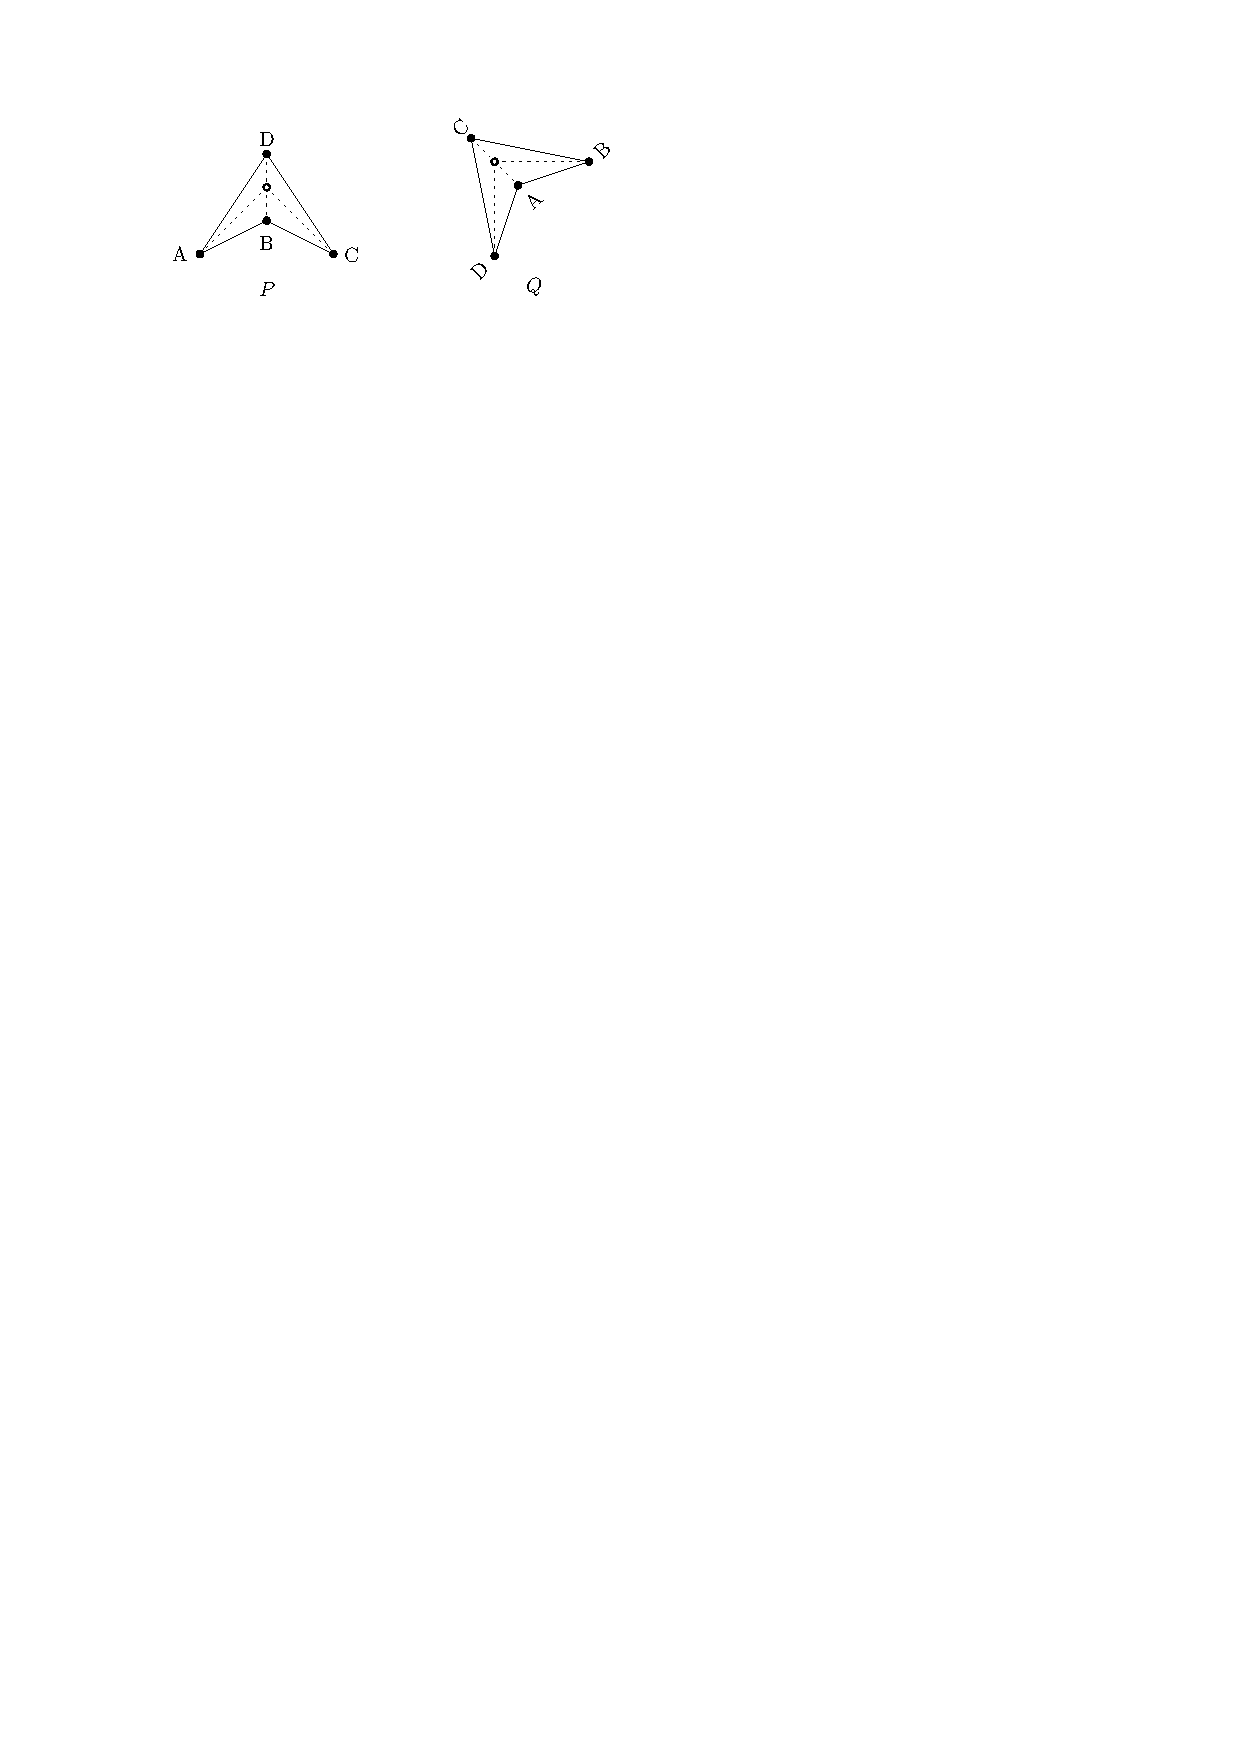
\includegraphics{img/compatible-triangs}
  }
  \caption{Compatible triangulations of two 4-gons $P$ and $Q$.}
  \label{fig:compatible-triangs}
\end{figure}

Babikov \etal\ \cite{babikov.souvaine.ea:constructing} showed that the result of Aronov \etal\ can be extended to polygons with holes. This work is the most closely related to ours because it encounters (the special case $k=2$ of) our problem as a subproblem. In their setting, the graph $\mathcal G$ is a collection of $r$ cycles, the embeddings $P$ and $Q$ are such that one cycle, $\mathcal C$, of $\mathcal G$ contains all the others in its interior and no other pair of cycles is nested in $P$ or $Q$. In the first stage of their algorithm, they build a connected supergraph $\mathcal{H}'$ of $\mathcal{G}$, but their supergraph has size $\Theta(n^2)$ in the worst case.  A byproduct of our main theorem is that this step of their algorithm could be done with a graph $\mathcal{H}'$ having only $O(nr^{1/2})$ edges (but completing this graph to a triangulation may still requires $\Omega(n^2)$ edges in the worst case).


\subsection{Outline}

To guide the reader, we give a rough sketch of our upper bound proof,
which is illustrated in Figure~\ref{figure:example}: For each component,
$\mathcal C_i$, of $\mathcal G$ we select a distinguished \emph{corner},
$a_i$, of $G_1$. (A corner is the space between two consecutive edges
incident on some vertex of the outer face). The corner $a_i$ is called
the \emph{attachment corner} for component $\mathcal C_i$.  Notice that,
since $G_1,\ldots,G_k$ are isomorphic, $a_i$ appears as a corner in each
of $G_1,\ldots,G_k$.

\begin{figure}
  \begin{center}
   \begin{tabular}{c}
     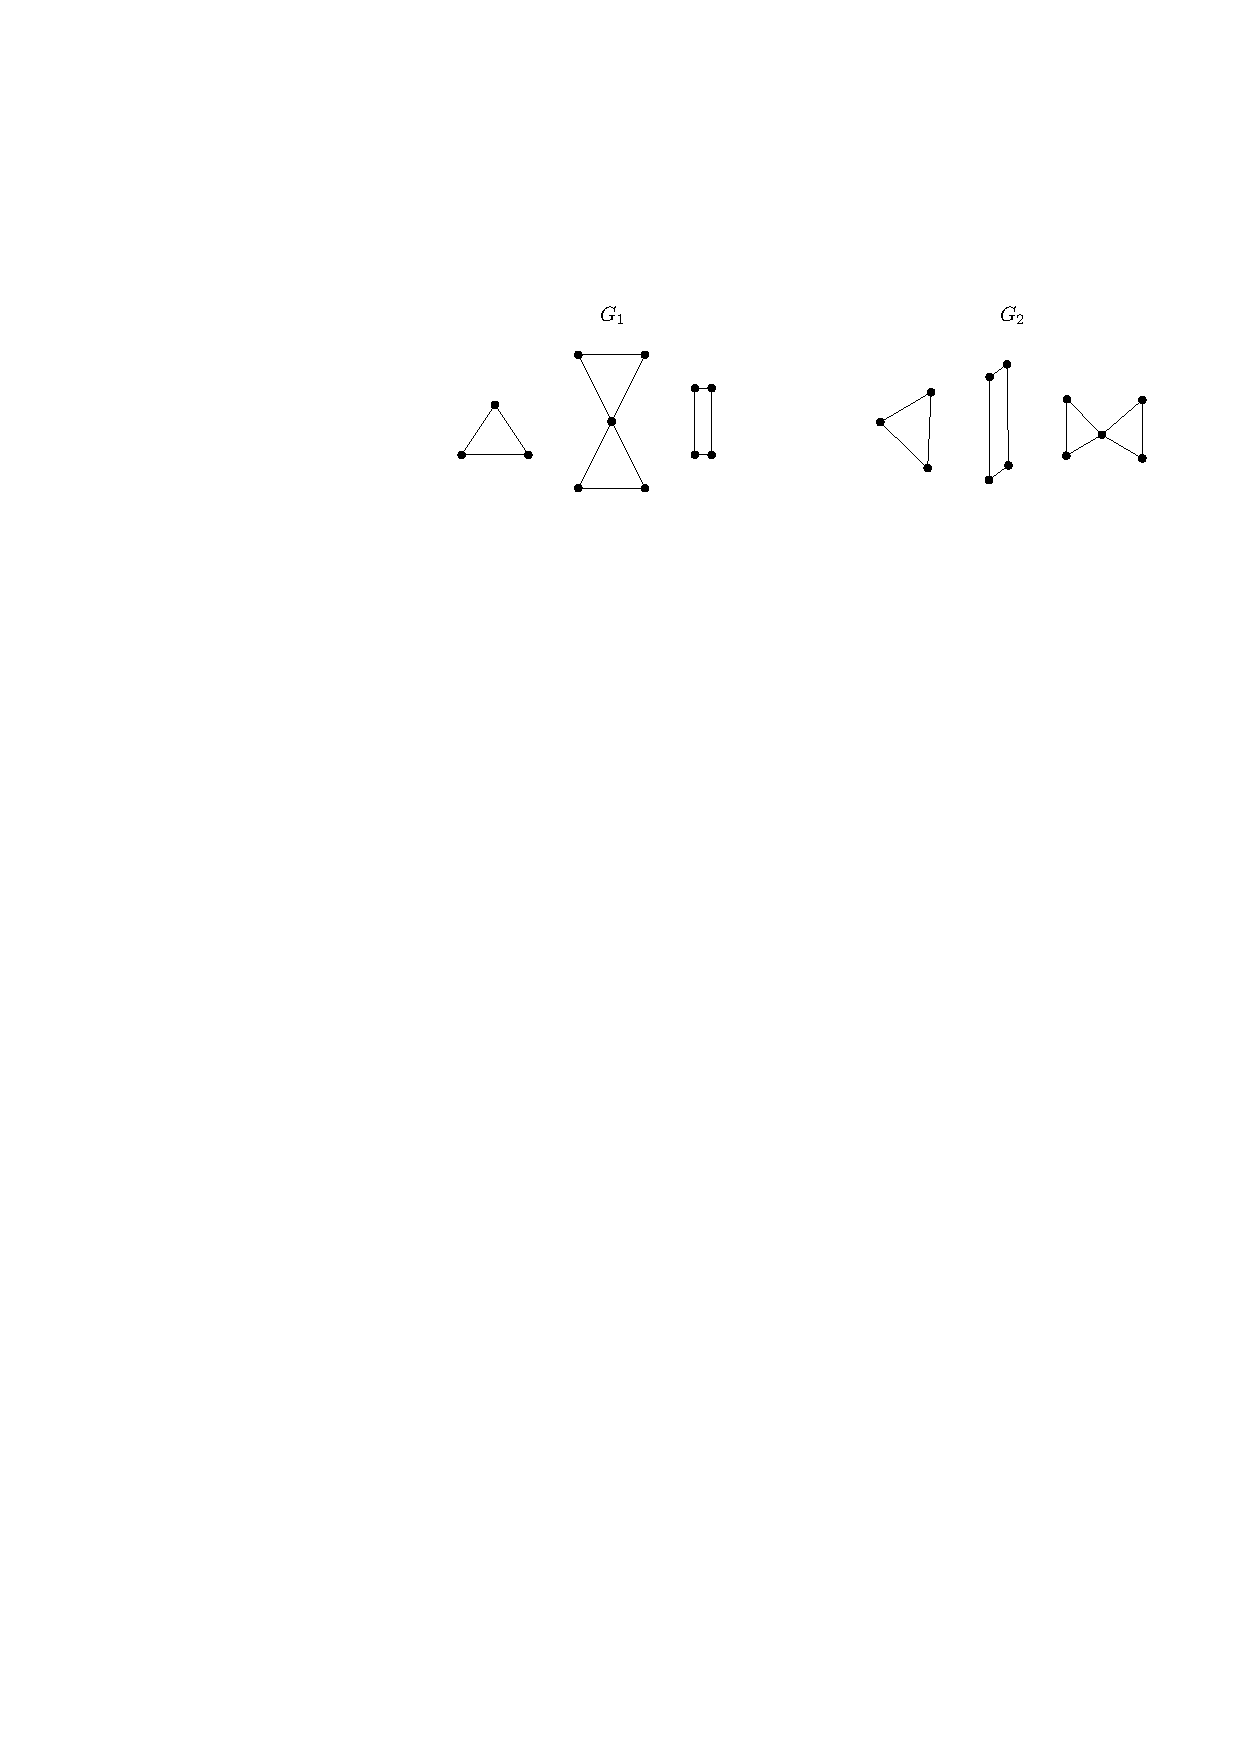
\includegraphics{img/example-1} \\[2ex]
     $\Downarrow$ \\
     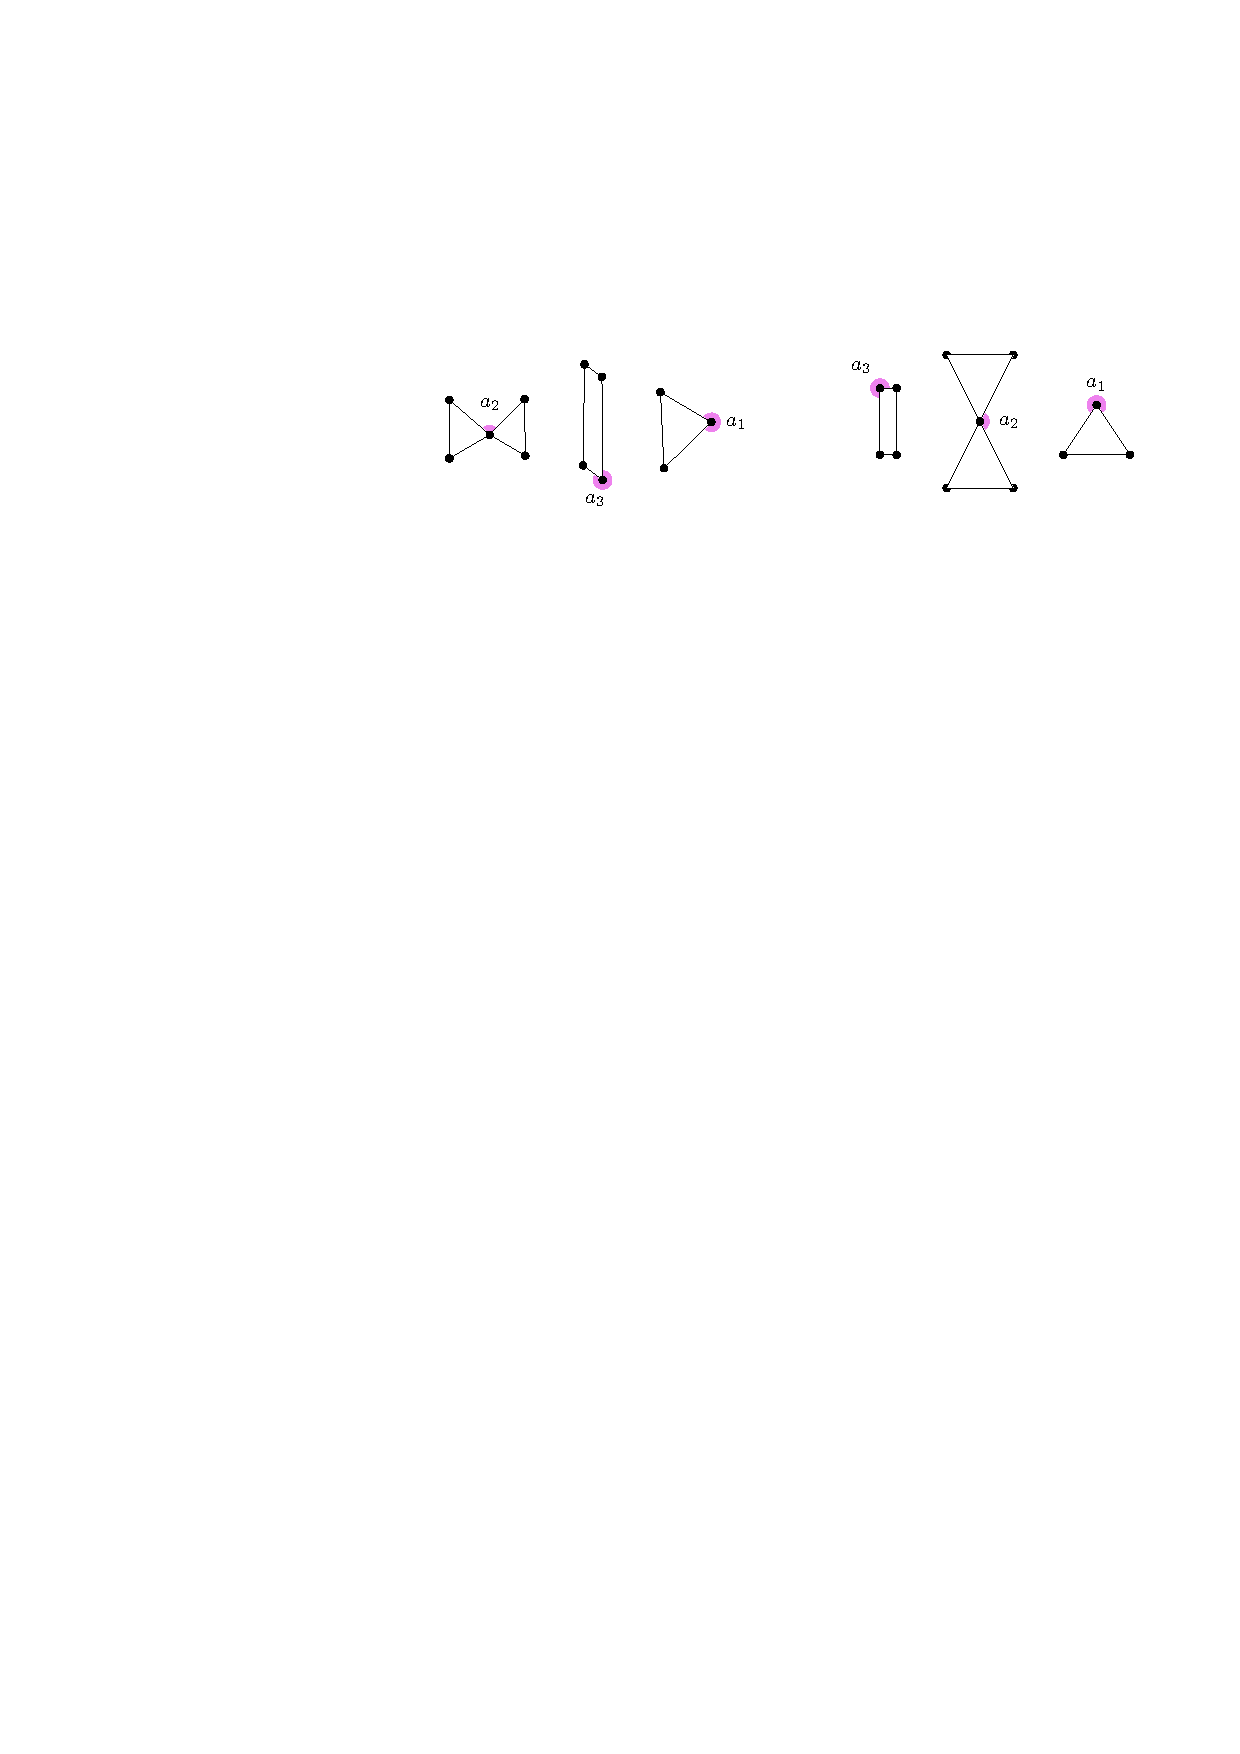
\includegraphics{img/example-2} \\[2ex]
     $\Downarrow$ \\
     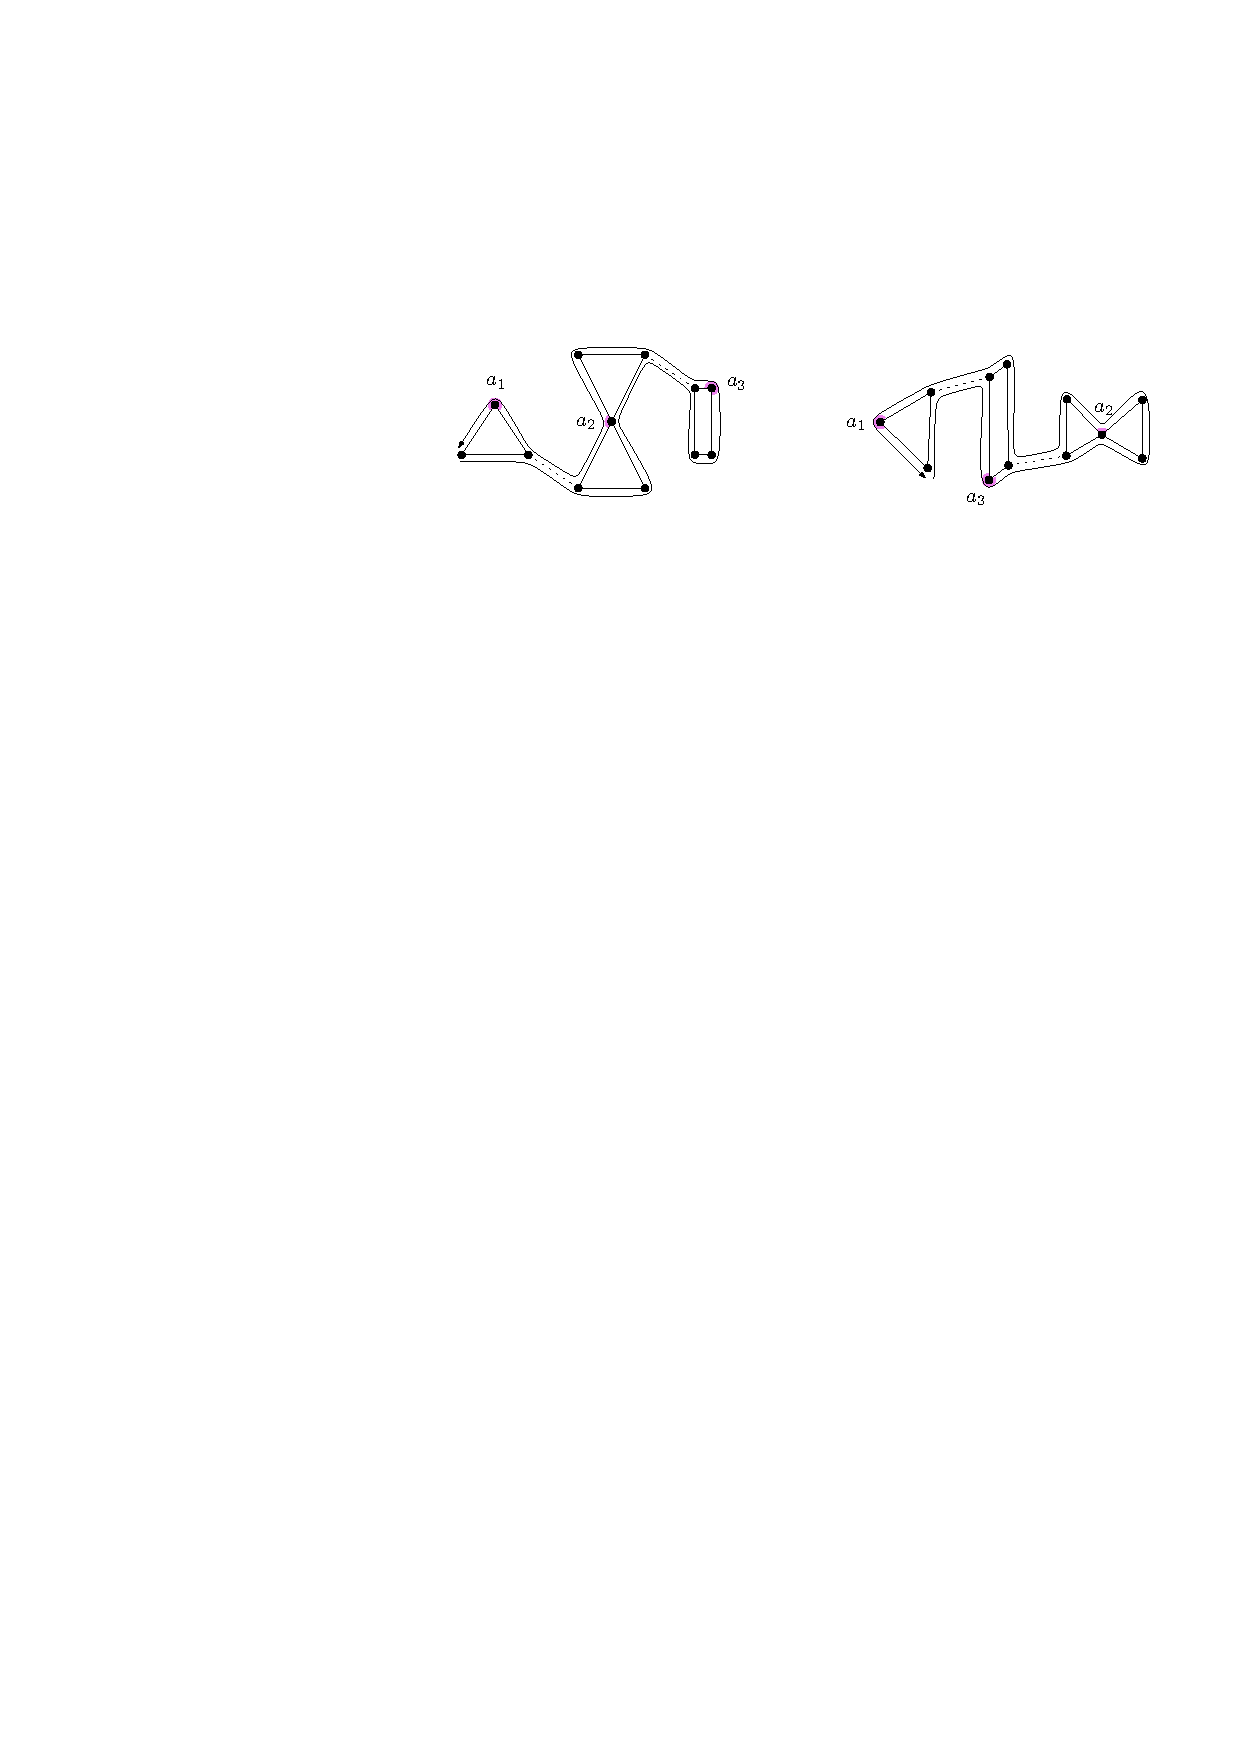
\includegraphics{img/example-3} \\[2ex]
     $\Downarrow$ \\
     Hamiltonian Path Algorithm Gives Path $a_3,a_2,a_1$ \\[2ex]
     $\Downarrow$ \\
     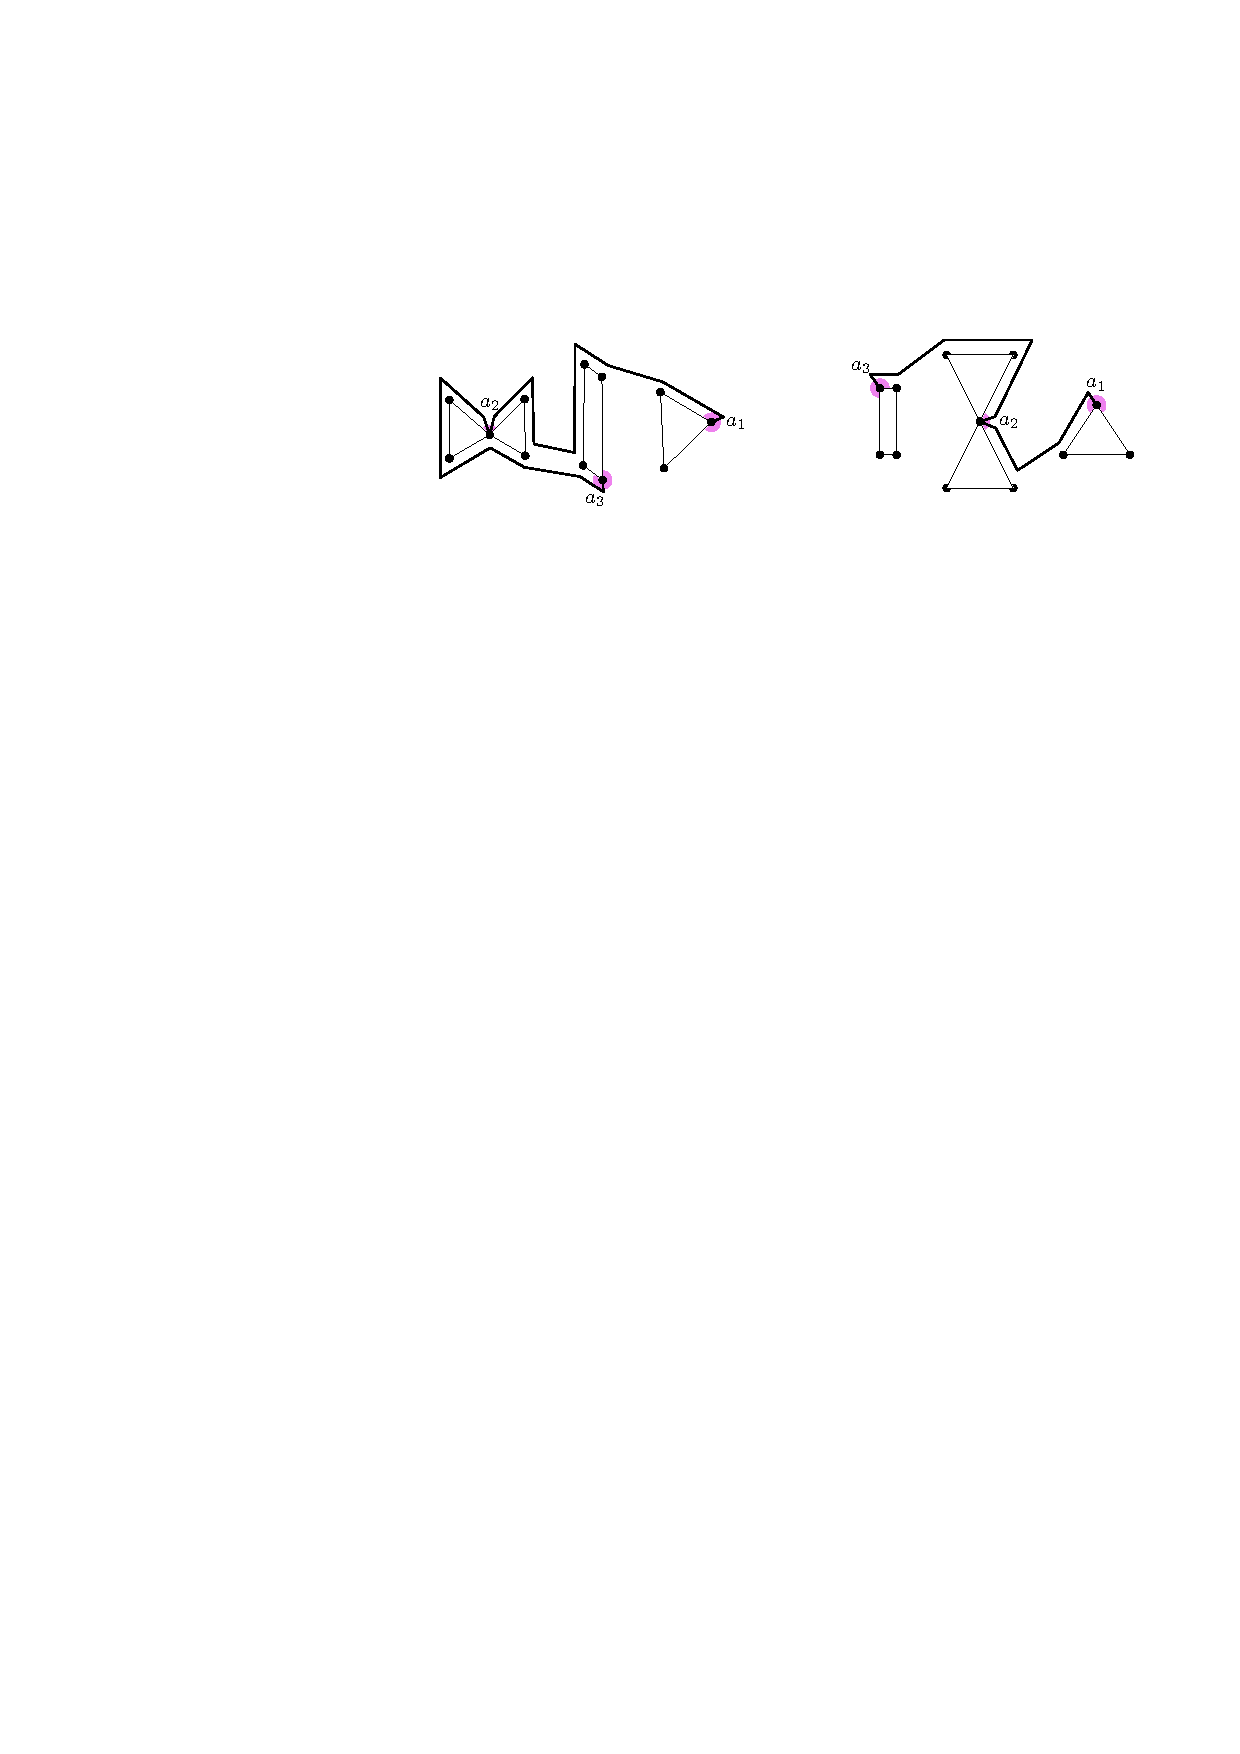
\includegraphics{img/example-4} 
   \end{tabular}
  \end{center}
  \caption{The algorithm for making a compatible augmentation of $\mathcal{G}$ works by defining corners $a_1,\ldots,a_r$, taking a spanning path on each embedding $G_i$ that visits all corners, and using this information to compute a permutation of $a_1,\ldots,a_r$ that can be embedded efficiently in each $G_i$.}
  \label{figure:example}
\end{figure}

Next, for each embedding, $G_j$, we add $r-1$ edges to make $G_j$ into a
connected graph, $G_j^*$.  We then traverse the boundary of the outer face
of $G_j^*$ to obtain a polygonal path, $\varphi_j$, of length $O(n)$ that comes
close to every corner of $G_j$.  The path $\varphi_j$ is then used to define an
integer distance $d_j(a_\ell,a_m)$ for any two corners $a_\ell$ and $a_m$. This distance includes information about the number of edges of $\varphi_j$ between $a_\ell$ and $b_m$ as well the sizes of the some of the components visited while walking from $a_\ell$ to $b_m$ along $\varphi_j$.

Next, we take a leap into $k$ dimensions by using the distance
functions $d_1,\ldots,d_k$ to produce an $k$-dimensional point set
$X=\{x_1,\ldots,x_r\}$ that lives in a hypercube of side-length $O(n)$.
This mapping has the property that, by adding a path of length $O(\|x_\ell
x_m\|)$ to $\mathcal G$, the corners $a_\ell$ and $a_m$ can be joined
in each of $G_1,\ldots,G_k$ while preserving planarity.

Now, since the point set $X$ is in $\R^k$, has $r$ points, and
lives in a hypercube of side-length $O(n)$, a result of Steele
and Snyder \cite{steele.snyder:worst} (see also Bern and Eppstein
\cite{bern.eppstein:worst}) implies that it has a spanning path of
Euclidean length $O(nr^{1-1/k})$.  This implies that $\mathcal G$ can be made
connected with a collection of $r-1$ paths, whose endpoints are the
corners $a_1,\ldots,a_r$, having total size $O(nr^{1-1/k})$, and
that each of these paths can be drawn in a planar fashion in each
of $G_1,\ldots,G_k$.

At this point, all that remains is to show that these $r-1$ paths
can each be drawn in each of $G_1,\ldots,G_k$ without crossing
each other.  This part of the proof involves carefully winding these
paths around the components in $G_1,\ldots,G_k$ using paths close
to the paths $\varphi_1,\ldots,\varphi_k$ defined above. This part
of the proof resembles the first part of the proof of Babikov \etal\
\cite{babikov.souvaine.ea:constructing}, but is complicated by the fact
that we have to be quite careful that the number of edges in these paths
remains in $O(nr^{1-1/k})$. 

In contrast to the upper bound, the lower-bound is quite simple and just
involves a sequence of nested paths whose vertices are the vertices of
a nested set of regular $\lfloor n/r\rfloor$-gons.

The remainder of the paper is organized as follows: In
Section~\ref{section:Trivial components} we start by solving
the special case in which the graph $G$ has no edges. This
special case is already non-trivial and introduces some of the
main ideas used in solving the full problem, which is tackled in
Section~\ref{section:General}. Section~\ref{section:Lower bound}
gives a simple lower bound construction that matches our upper bound
for all values of $r$, $n$, and $k$.  
%The paper concludes with
%Section~\ref{section:Conclusions}, which summarizes and presents
%directions for future research.


%%%%%%%%%
\section{Upper bounds for trivial components}\label{section:Trivial components}
As a warmup, we consider a graph containing $n$ vertices and no edges,
i.e., a graph that consists of $n$ (trivial) connected components.
Before constructing the compatible augmentation, we provide a subroutine
that constructs a ``short'' plane spanning path of a point set that
connects the points in a prescribed order.

\subsection{Spanning paths of point sets}
Let $S$ be a set of $n$ points in the plane such that no two points of $S$ have the same $x$-coordinate. 
Given a point $v\in S$, let $\rank(v)$ denote the number of points of $S$ that lie to the left of (having smaller $x$-coordinate than) $v$.

Given an arbitrary order $(v_1, v_2, \ldots, v_n)$ of the points of $S$, we want to construct a path $R$ that connects them in this order and such that:  
\[
   |R|  = O\left(\sum_{i=1}^{n-1} |\rank(v_i) - \rank(v_{i+1})| \right).
\]
(This paper (over-)uses the $|\cdot|$ operator in several different ways, depending on the type of its argument.  For a real number, $x$, $|x|$ is the absolute value of $x$.  For a walk, $R=(r_0,\ldots,r_k)$, $|R|=k$ denotes the number of edges traversed by $R$. For a (weakly-)simple polygon, $P$ whose vertices---as encountered during a counterclockwise traversal---are $(a_1,\ldots,a_k)$, $|P|=k$, the number of edges of $P$.)

Consider a horizontal line such that each point of $S$ lies above it and let $\pi$ be the closed halfspace supported by this line that contains $S$.  We present an algorithm that constructs the path in $R$ in rounds; during the $i$th round, the path is extended to include $v_i$.  After each round of the algorithm, we maintain the invariant that the boundary of $\pi$ does not intersect $R$.

Throughout, we also maintain the \emph{escape invariant} which states that for each point $v_j\in S \setminus R$, there is a cone $\Delta_j$ with apex $u_j$ such that (1) $u_j$ lies above $v_j$ (or on $v_j$) and has the same $x$-coordinate as $v_j$, (2) $\Delta_j$ contains $v_j$ and no other point of $S$, (3) $\Delta_j$ contains the ray originating at $v_j$ in the direction of the negative $y$-axis, (4) $\Delta_j$ does not intersect $R$, and (5) $\Delta_i$ and $\Delta_j$ are disjoint inside $\pi$.
Before starting the construction, we establish the escape invariant. To do this, for each $0\leq j\leq n$ let $u_j$ be an arbitrary translation of $v_j$ in the direction of the positive $y$-axis and let $\Delta_j$ be a cone with apex on $u_j$ sufficiently narrow such that these cones doe not intersect inside $\pi$; see Figure~\ref{fig:Escape Invariant}.

\begin{figure}[tb]
\centering 
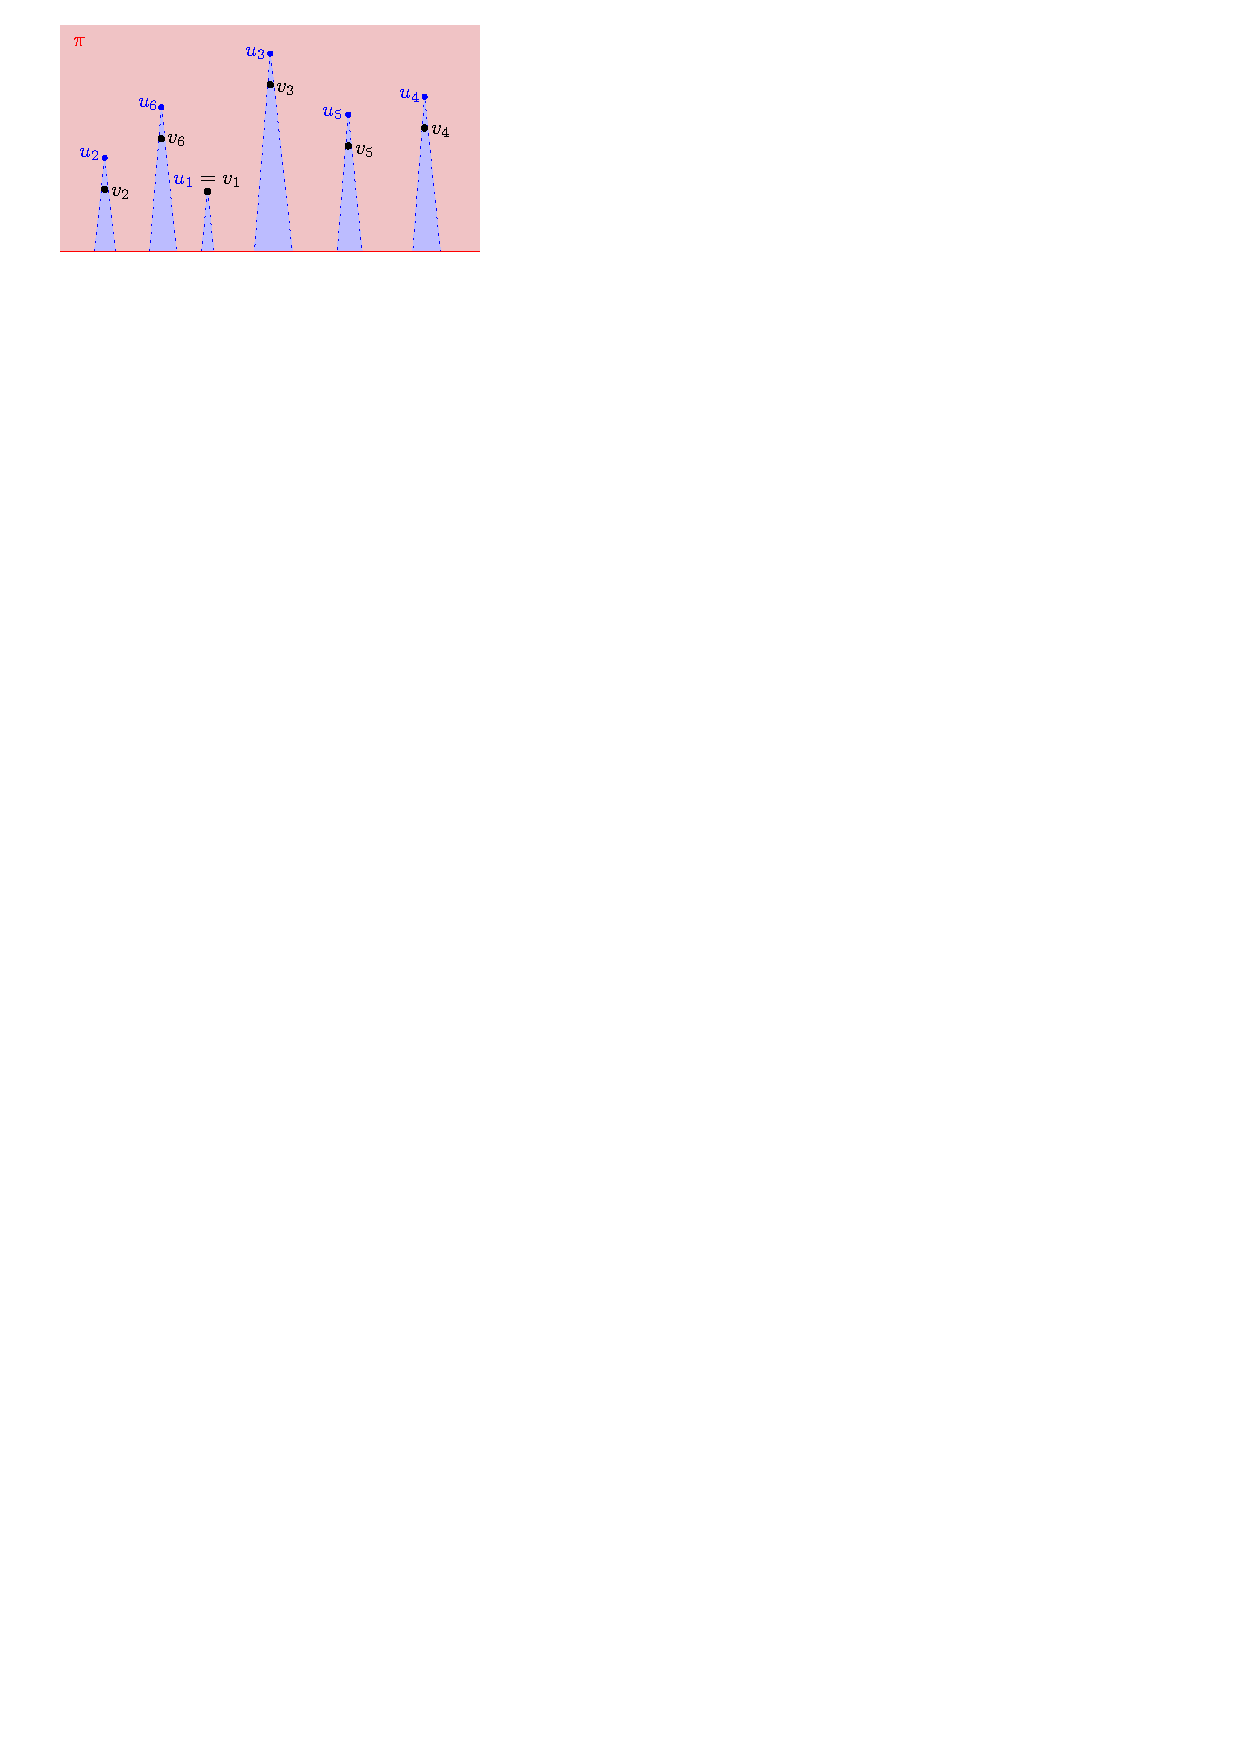
\includegraphics{img/EscapeInvariant.pdf}
%[width=1\textwidth]
\caption{The halfplane $\pi$ and the cones $\Delta_1,\ldots,\Delta_n$ with apexes at $u_1,\ldots,u_n$.}
\label{fig:Escape Invariant}
\end{figure}

To construct $R$, we add the points of $S$, one by one, according to
the given order while maintaining the escape invariant.  Assume that
$R$ is a path connecting $v_1$ with $v_j$. (Initially, $j=1$ and $R$
consists of the single vertex $v_1$).  We extend $R$ by appending a
path that connects $v_j$ with $v_{j+1}$.  As a first step, we translate
down the cones $\Delta_j$ and $\Delta_{j+1}$ until their apexes $u_j$
and $u_{j+1}$ coincide with $v_j$ and $v_{j+1}$, respectively.
\red{Pat says: I removed a narrowing operation here that isn't necessary if
we shift both $\pi$ and $u_{j+2},...,u_n$ downward simultaneously.}
% Pat says: I don't think this is necessary since we're shifting both $\pi$ and $u_{j+2},...,u_n$ downward:
% Moreover, we narrow the cone $\Delta_j$ while keeping the ray originating downwards from $v_j$ contained in $\Delta_j$.

Let $\pi_j$ be the closure of the set obtained from $\pi$ by removing the cone $\Delta_h$, for every $h\in\{j,j+1,\ldots,n\}$; see Figure~\ref{fig:Dented Halfspace}. That is, $\pi_j$ is a halfspace with dents made by the removal of $n-j+1$ cones.
%Therefore, the number of segments on the boundary of $\pi_j$ is $O(n-j)$. 
Observe that, for every pair of apexes $u_i$ and $u_h$, the boundary of $\pi_j$
contains a path from $u_i$ to $u_h$ consisting of $O(|\rank(v_i)-\rank(v_j)|)$ edges.

\begin{figure}[tb]
\centering
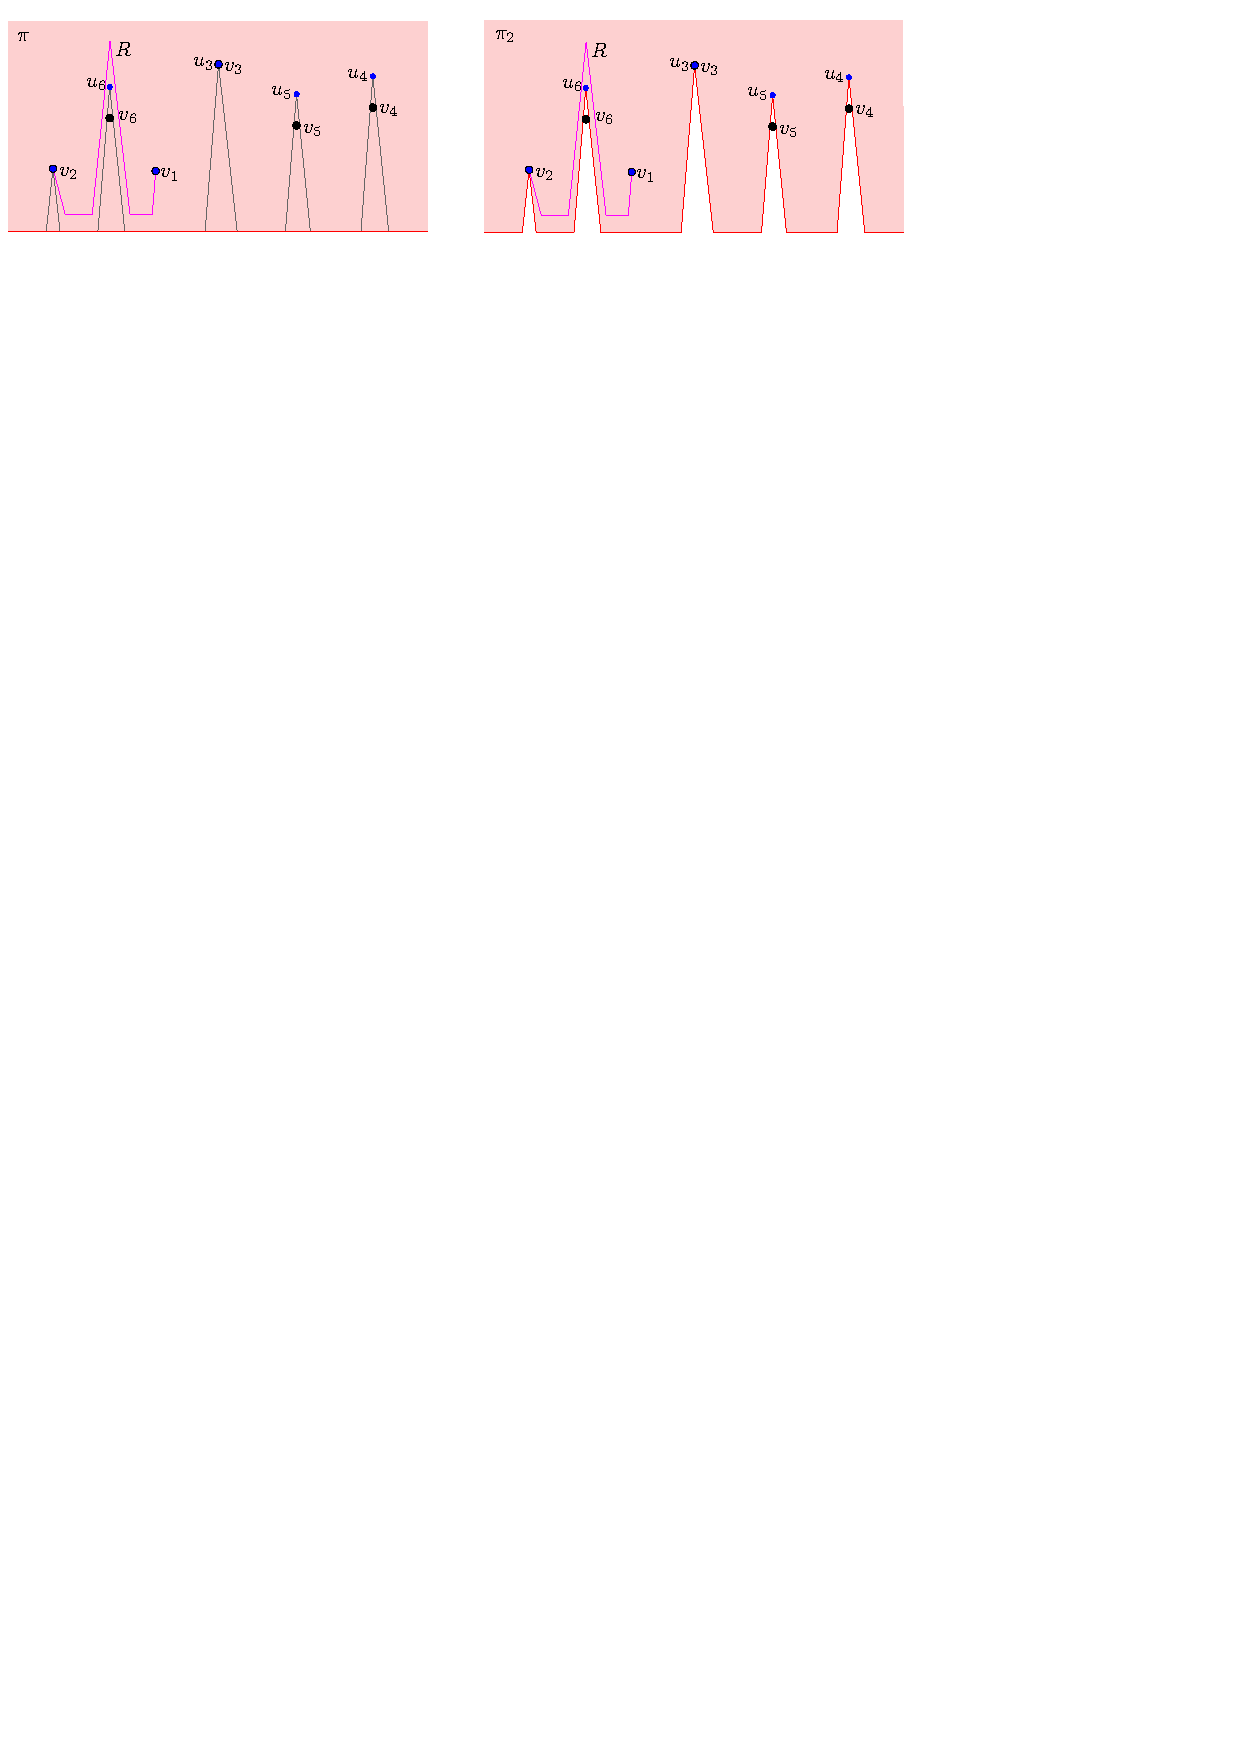
\includegraphics[width=.98\textwidth]{img/DentedHalfspace.pdf}
\caption{The boundary of $\pi_2$ is in the path from $v_2$ to $v_3$.}
\label{fig:Dented Halfspace}
\end{figure}

Because the boundary of $\pi$ does not intersect $R$ and by property (4) of the escape invariant, the boundary of $\pi_j$ intersects the portion of $R$ constructed so far only at $v_j$. Moreover, by property (2) of the escape invariant, each point of $S\setminus V(R)$ lies outside of~$\pi_j$ except for $v_{j+1}$ that lies on its boundary.
Because both $v_j$ and $v_{j+1}$ lie on the boundary of $\pi_j$ and since this boundary does not intersect the interior of $R$, we can connect $v_j$ with $v_{j+1}$ with a path contained in the boundary of $\pi_j$. 
Recall that this path has length $O(|\rank(v_j) - \rank(v_{j+1})|)$. In this way, we extend $R$ to a planar path that connects $v_1$ with $v_{j+1}$.

After connecting $v_j$ with $v_{j+1}$, for each $h\in\{j+2,\ldots,n\}$, either $\Delta_h$ is disjoint from $R$, or it shares some portion of its boundary with $R$. However, the interior of $\Delta_h$ does not intersect $R$.
To preserve the escape invariant, we translate $\pi$ and $\Delta_h$, for each $h\in\{j+1,\ldots,n\}$ downward by a sufficiently small amount, $\varepsilon$. Because each translated cone is contained in the previous one and since its apex $u_h$ lies above $v_h$ by property (1) of the escape invariant, by choosing $\varepsilon$ sufficiently small, we guarantee that the escape invariant is maintained.  Thus, the algorithm is ready to proceed to the next round and doing this $n-1$ times gives the following result.

\begin{lemma}\label{lemma:Compatible augmentation for trivial components}
Given an arbitrary order $(v_1, \ldots, v_n)$ of the vertices of $S$, the previous algorithm computes a plane path $R$ that connects every point of $S$ in the given order such that 
$|R| = O\left(\sum_{i=1}^{n-1} |\rank(v_i) - \rank(v_{i+1})| \right)$. 
\end{lemma}
\begin{proof}
Recall that in each iteration, the algorithms computes a path connecting $v_j$ with $v_{j+1}$ that does not cross the portion of the path already constructed. Because this invariant is maintained throughout, the resulting path is planar.

Since the path that connects $v_j$ with $v_{j+1}$ follows the boundary of $\pi_j$ and since this boundary has length $O(|\rank(v_j) - \rank(v_{j+1})|)$ between $v_j$ and $v_{j+1}$, the path that connects $v_j$ with $v_{j+1}$ has length $O(|\rank(v_j) - \rank(v_{j+1})|)$. Consequently,  the total length of $R$ is given by $O\left(\sum_{i=1}^{n-1} |\rank(v_i) - \rank(v_{i+1}) |\right)$.
\end{proof}



\subsection{Compatible drawings of point sets}
Recall that in this section, $\mathcal G$ is a graph with $n$ trivial components.
Let $G_1, \ldots, G_k$ be $k$ isomorphic drawings of $\mathcal G$, i.e., $G_i$ is a set of $n$ points in the plane.
Assume without loss of generality that no two points of $G_i$ share the same $x$-coordinate. Otherwise, rotate the coordinate system slightly.
Given a vertex $v$ of $\mathcal G$, let $\rank_{G_i}(v)$ denote the number of points of $G_i$ to the left of $v$.

For each $v$ of $\mathcal G$, let $x_v = (\rank_{G_1}(v), \rank_{G_2}(v),
\ldots, \rank_{G_k}(v))$ be a point in the integer grid of side-length
$n$ contained in $\mathbb{R}^k$.  Let $X = \{x_v : v\in V(\mathcal G)\}$
and let $P$ be the Euclidean shortest Hamiltonian path of $X$, i.e., the shortest
path that visits every point of $X$.  It is known that the length of
$P$ is $O(n^{2-1/k})$~\cite{steele.snyder:worst}. 
Note that the order of the points of $P$ induces an order on the vertices of $\mathcal G$ and hence, an order on the points of each $G_i$. 


\begin{theorem}\label{theorem:points}
For each $1\leq i\leq n$, we can construct a path $R_i$ of length $O(n^{2-1/k})$ that connects every point of $G_i$ such that $G_i\cup R_i$ is plane. Moreover, for each $1\leq i < j \leq n$, $G_i\cup R_i$ is isomorphic to $G_j\cup R_j$.
\end{theorem}
\begin{proof}
By relabelling, let $(v_1, \ldots, v_n)$ denote the order of the vertices
of $\mathcal{G}$ induced by $P$.  The augmented graph $\mathcal{H}$
is a path that visits the vertices $v_1,\ldots,v_n$ in this order.
Letting $d_j$ denote the distance between $x_{v_j}$ and $x_{v_{j+1}}$,
the path $\mathcal{H}$ includes an addition $O(d_j)$ vertices between
$v_{j}$ and $v_{j+1}$.  It immediately follows that the number of vertices
in $\mathcal{H}$ is proportional to the length of $P$, which is $O(n^{2-1/k})$.

Next, for each $G_i$, we use Lemma~\ref{lemma:Compatible augmentation
for trivial components} to draw $\mathcal{H}$ as a plane path, $R_i$,
that connects the vertices $v_1,\ldots,v_n$ in the drawing $G_i$.
Since $d_j\ge |\rank_{G_i}(v_j) - \rank_{G_i}(v_{j+1})|$, the $O(d_j)$
vertices in $\mathcal{H}$ between $v_j$ and $v_{j+1}$ are enough to
draw the $O(|\rank_{G_i}(v_j) - \rank_{G_i}(v_{j+1})|)$ vertices in $R_i$
between $v_j$ and $v_{j+1}$.

Since the vertices of each $G_i$ are connected in the same order,
$G_i\cup R_i$ is isomorphic to $G_j\cup R_j$ for each $i,j\in\{1,\ldots,k\}$.
\end{proof}


\section{The general problem}\label{section:General}
In this section, we extend the result presented in
Section~\ref{section:Trivial components} to graphs with
non-trivial components.  We follow the same general scheme used in
Section~\ref{section:Trivial components} for the case of trivial
(isolated vertex) components:  We define $k$ different
orderings on the components of $\mathcal G$ and use these orderings (and
the sizes of these components) to define an $r$-point set, $X$, in $\R^k$. A
short path that visits all points in $X$ is then translated back into
a short path, $R$, that visits each component of $\mathcal G$. The path
$R$ is then 
added, as a polygonal path, $R_i$, to each drawing, $G_i$, of $\mathcal G$.

Things are somewhat more complicated because, unlike the case in which
components are isolated vertices, there is no natural ordering of the
components of $G_i$, so we must define one. Next, the drawing
of the path $R_i$ is considerably more complicated.  In the Section~\ref{section:Trivial components}, $R_i$ is drawn incrementally and always passes above components that are not yet included in $R_i$ and passes below components that are already included in $R_i$.  In this section, we have to find meaningful definition of ``above'' and ``below'' and be quite careful because the costs of going ``above'' or ``below'' components depends on the size and structure of those components.

We begin with some careful definitions because, when a component is not an
isolated vertex, we have to be considerably more specific about how the
path, $R$, to it.


\subsection{Preliminaries}\label{section:Preliminaries} 
Let $C$ be a connected geometric plane graph. Let $v_0, v_1, \ldots, v_k, v_0$ be the sequence of vertices of $C$ visited by a counterclockwise
Eulerian tour along the boundary of the outer face of $C$. Note that
$v_i$ may be equal to $v_j$ for some $i\neq j$.  A vertex of $v_i$
in this sequence is called a \emph{corner} of $C$.  In this paper,
we consider the boundary of $C$, denoted by $\partial C$, to be the
boundary of the weakly-simple polygon $(v_0, \ldots, v_k, v_0)$ whose
vertex set is the set of corners of $C$.\footnote{More formally, $\partial C$ is the boundary of the unbounded component of $\mathbb{R}^2\setminus C$, where we treat $C$ as the union of all its edges and vertices.}  

Let $\varepsilon >0$. For each corner $v_i$ of $\partial C$,
let $\ell_i$ be the line passing through $v_i$ that bisects the angle between the edges $v_{i-1}v_i$ and $v_i v_{i+1}$.
Let $z_i$ be the point at distance $\varepsilon$ from $v_i$ along $\ell_i$ such that $v_{i-1} v_i z_i$ either makes a right turn or defines three collinear points such that $v_i\in [v_{i-1}, z_i]$. We call $z_i$ the \emph{$\varepsilon$-copy} of $v_i$.
Let $\partial_\varepsilon C$ be the polygon defined by the sequence $(z_0, z_1, \ldots, z_k, z_0)$, i.e., $\partial_\varepsilon C$ is isomorphic to $\partial C$ (but not necessarily to $C$). We call $\partial_\varepsilon C$ the \emph{$\varepsilon$-fattening} of $C$.
An $\varepsilon$-fattening $\partial_\varepsilon C$ is \emph{simple} if $\partial_\varepsilon C$  is a simple polygon that contains~$C$.
Note that $\partial_\varepsilon C$ is simple, provided that $\varepsilon$ is sufficiently small. In this paper, we consider only simple $\varepsilon$-fattenings; see Figure~\ref{fig:Blowing}. Note that the (graph) distance between two corners of $\partial C$ along the boundary of $C$ is the same as the distance between their $\varepsilon$-copies along~$\partial_\varepsilon C$.

%%%%%%%%%%%%%%%
\subsection{Connected augmentations}\label{section: connected augmentations}
Let $G$ be a geometric plane graph with $r$ connected components such that each component is adjacent to the outer face.
Consider the visibility graph of $G$ where two vertices are visible if the open segment joining them does not intersect $G$.
Let $T_G$ be a smallest set of edges of the visibility graph of $G$ that need to be added to $G$ to make it connected.
Because there are always two components visible from each other, we can connect them and repeat recursively with one less component.  This implies that $T_G$ has $r-1$ edges. (Loosely, we can think of $T_G$ as a spanning tree of $G$'s components.) Let $G^* = G\cup T_G$.  We say that $G^*$ is a \emph{connected augmentation} of $G$; see Figure~\ref{fig:Blowing}.

\begin{figure}[tb]
\centering
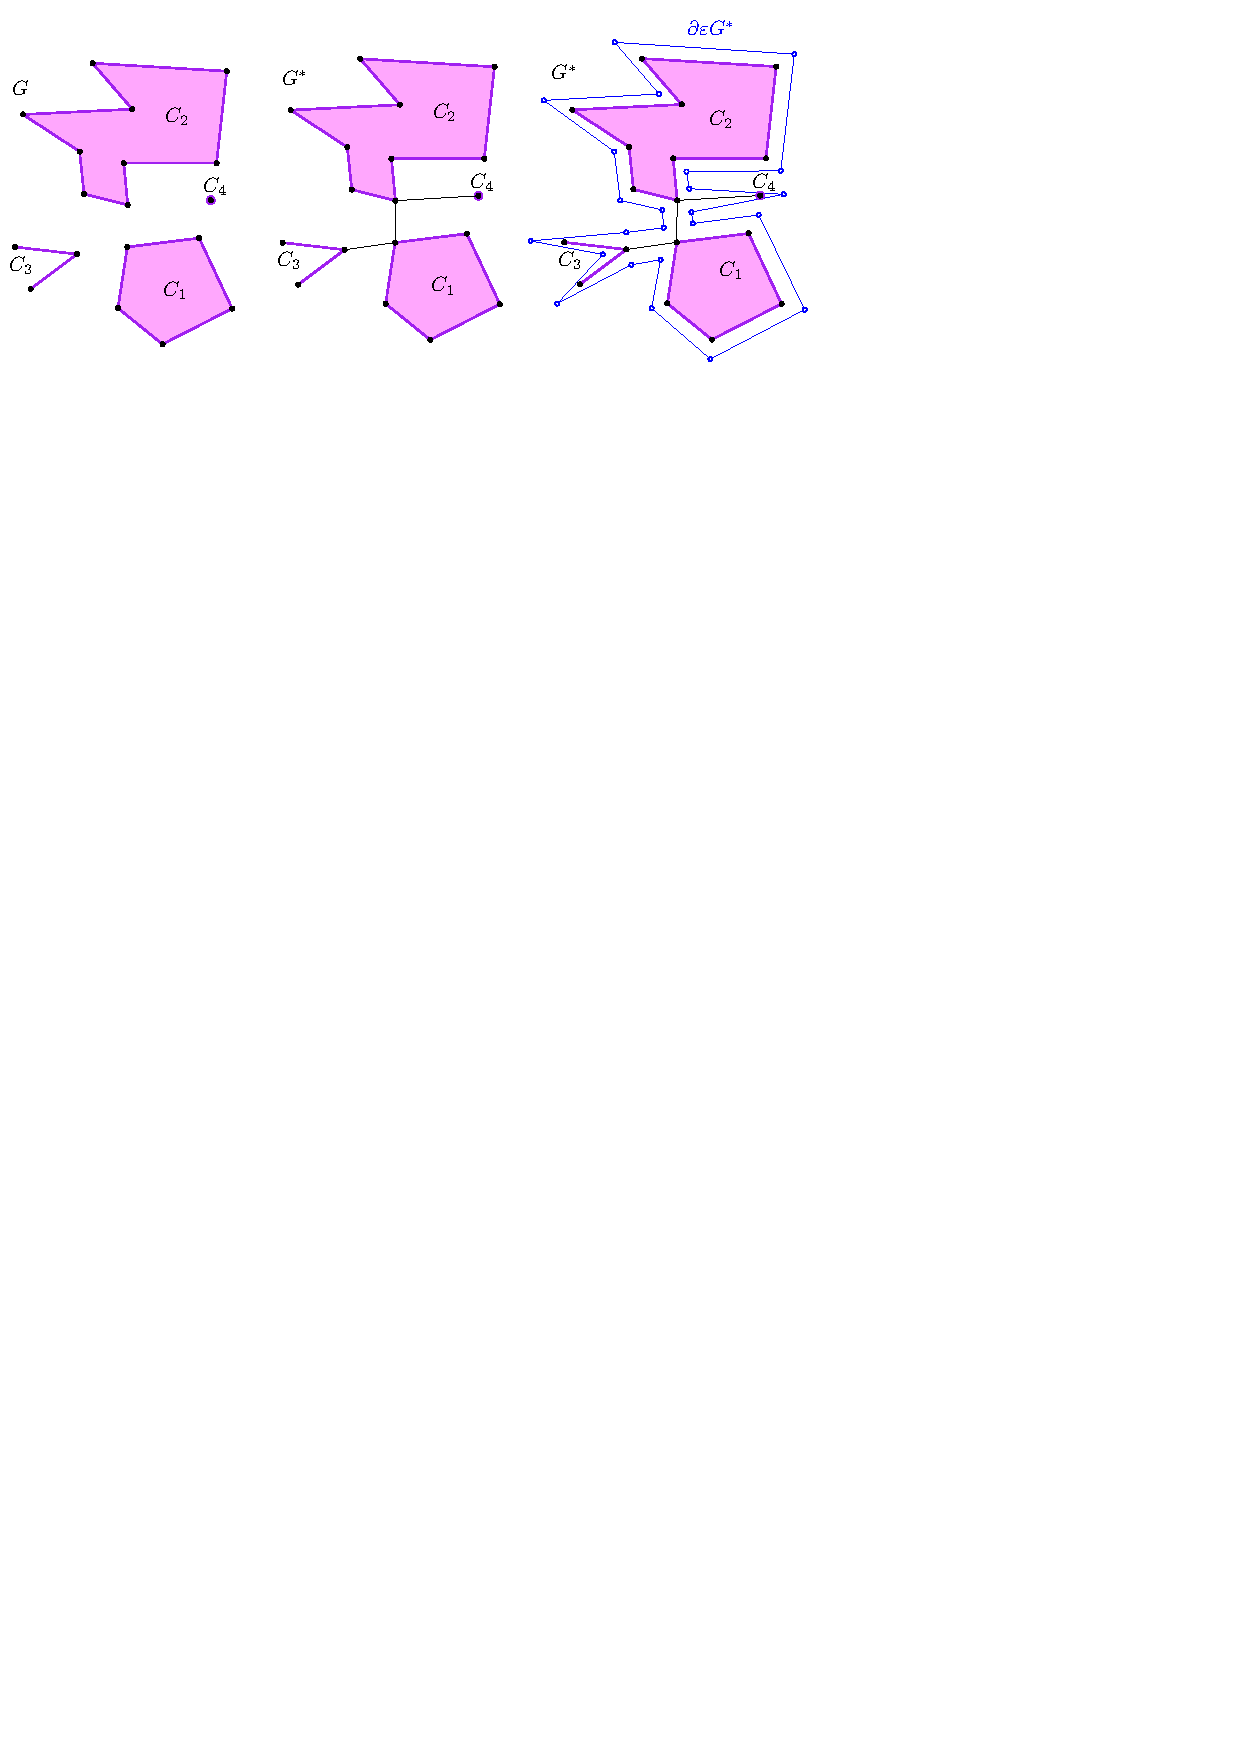
\includegraphics{img/Blowing.pdf}
%[width=1\textwidth]
\caption{The graph $G$ (left); a connected augmentation, $G^*$, of $G$ (middle); and the $\varepsilon$-fattening, $\partial_\varepsilon G^*$ (right).}
\label{fig:Blowing}
\end{figure}

Let $C_1, \ldots, C_r$ be the components of $G$. 
Recall that we consider $\partial C_i$ to be the boundary of a weakly-simple polygon. Therefore, even though a vertex of $C_i$ can appear multiple times along $\partial C_i$, we consider them as different corners of $\partial C_i$. 
For each $1\leq i\leq r$, let $a_i\in C_i$ be an arbitrary corner of $\partial C_i$ (note that $a_i$ is adjacent to the outer face).
We call $a_i$ the \emph{attachment corner} of $C_i$.

Let $\varphi$ be the path obtained by splitting $\partial G^*$ at the corner $a_1$. 
That is, $\varphi$ is a path with both endpoints equal to $a_1$. 
Note that $\varphi$ visits every corner of $\partial G^*$ exactly once except for $a_1$.
Given two corners $u$ and $v$ in $\partial G^*$, let $\varphi(u,v)$ denote
the unique path in $\varphi$ that connects $u$ with $v$. Let $A(u,v)$ be
the set of attachment corners of $G$ visited by $\varphi(u,v)$. Define 
\[
     \sigma_G(u,v) = |\varphi(u,v)| + \sum_{a_i\in A(u,v)}|\partial C_i| \enspace ,
\]
which we call the \emph{cost} of going from $u$ to $v$.

\begin{lemma}\label{lemma:Contained in integer grid}
  If $a$ is an attachment corner of $G$, then $\sigma_G(a_1, a) \leq
  4n$. Moreover, if $b$ is another attachment corner of $G$, then
  $\sigma_G(a, b) =  |\sigma_G(a_1, a)- \sigma_G(a_1, b)|$.
\end{lemma}
\begin{proof}
Recall that $G^*$ is a graph with $n$ vertices, so $\partial G^*$ is a weakly-simple polygon with at most $n$ distinct vertices, so $|\partial G^*|\le 2n-2<2n$.
Furthermore, $\varphi(a_1,a)\subset \partial G^*$, so
$|\varphi(a_1,a)|\le |\partial G^*|< 2n$.  Similarly, $\sum_{a_i\in A(a_1,a)} \le \sum_{i=1}^r |\partial C_i| < 2n$.
Therefore, $\sigma_G(a_1,a)< 4n$, which is the first part of the lemma.

To prove the second part of the lemma, 
assume without loss of generality that $a$ is visited before $b$ by $\varphi$.
We immediately have that $\varphi(a,b)=\varphi(a_1,b)\setminus\varphi(a_1,a)$.
Furthermore, since each attachment corner of $G$ visited by $\varphi(a_1, a)$ is also visited by $\varphi(a_1, b)$, we have that $A(a,b)=A(a_1,b)\setminus A(a_1,a)$.  So we get
$\sigma_G(a_1, b)- \sigma_G(a_1, a) = |\sigma_G(a_1, a) - \sigma_G(a_1, b)| = |\varphi(a, b)|  + \sum_{a_i\in A(a, b)} |C_i| = \sigma_G(a, b)$.
\end{proof}

\subsection{Spanning paths for connected augmentations}\label{section:Spanning paths for connected augmentations}
Let $a_1, \ldots, a_r$ be an arbitrary order of the attachment corners of $G$ (we can get the incremental indexing by relabeling the components). 
Given a path $R = (\rho_1, \rho_2, \ldots, \rho_t)$ that passes through all attachment corners of $G$, we say that $C_i$ lies to the right of $R$ if (1) $a_i$ is the only vertex of $C_i$ that belongs to $V(R)$, and (2) if $a_i = \rho_j$ for some $j\in\{1,\ldots,t\}$, then $\rho_{j-1}$ and $\rho_{j+1}$ appear as consecutive vertices when sorting---in the graph $G\cup R$---the neighbors of $a_i$ in clockwise order around $a_i$ (see Figure~\ref{figure:right-of}).


\begin{figure}
\centering
  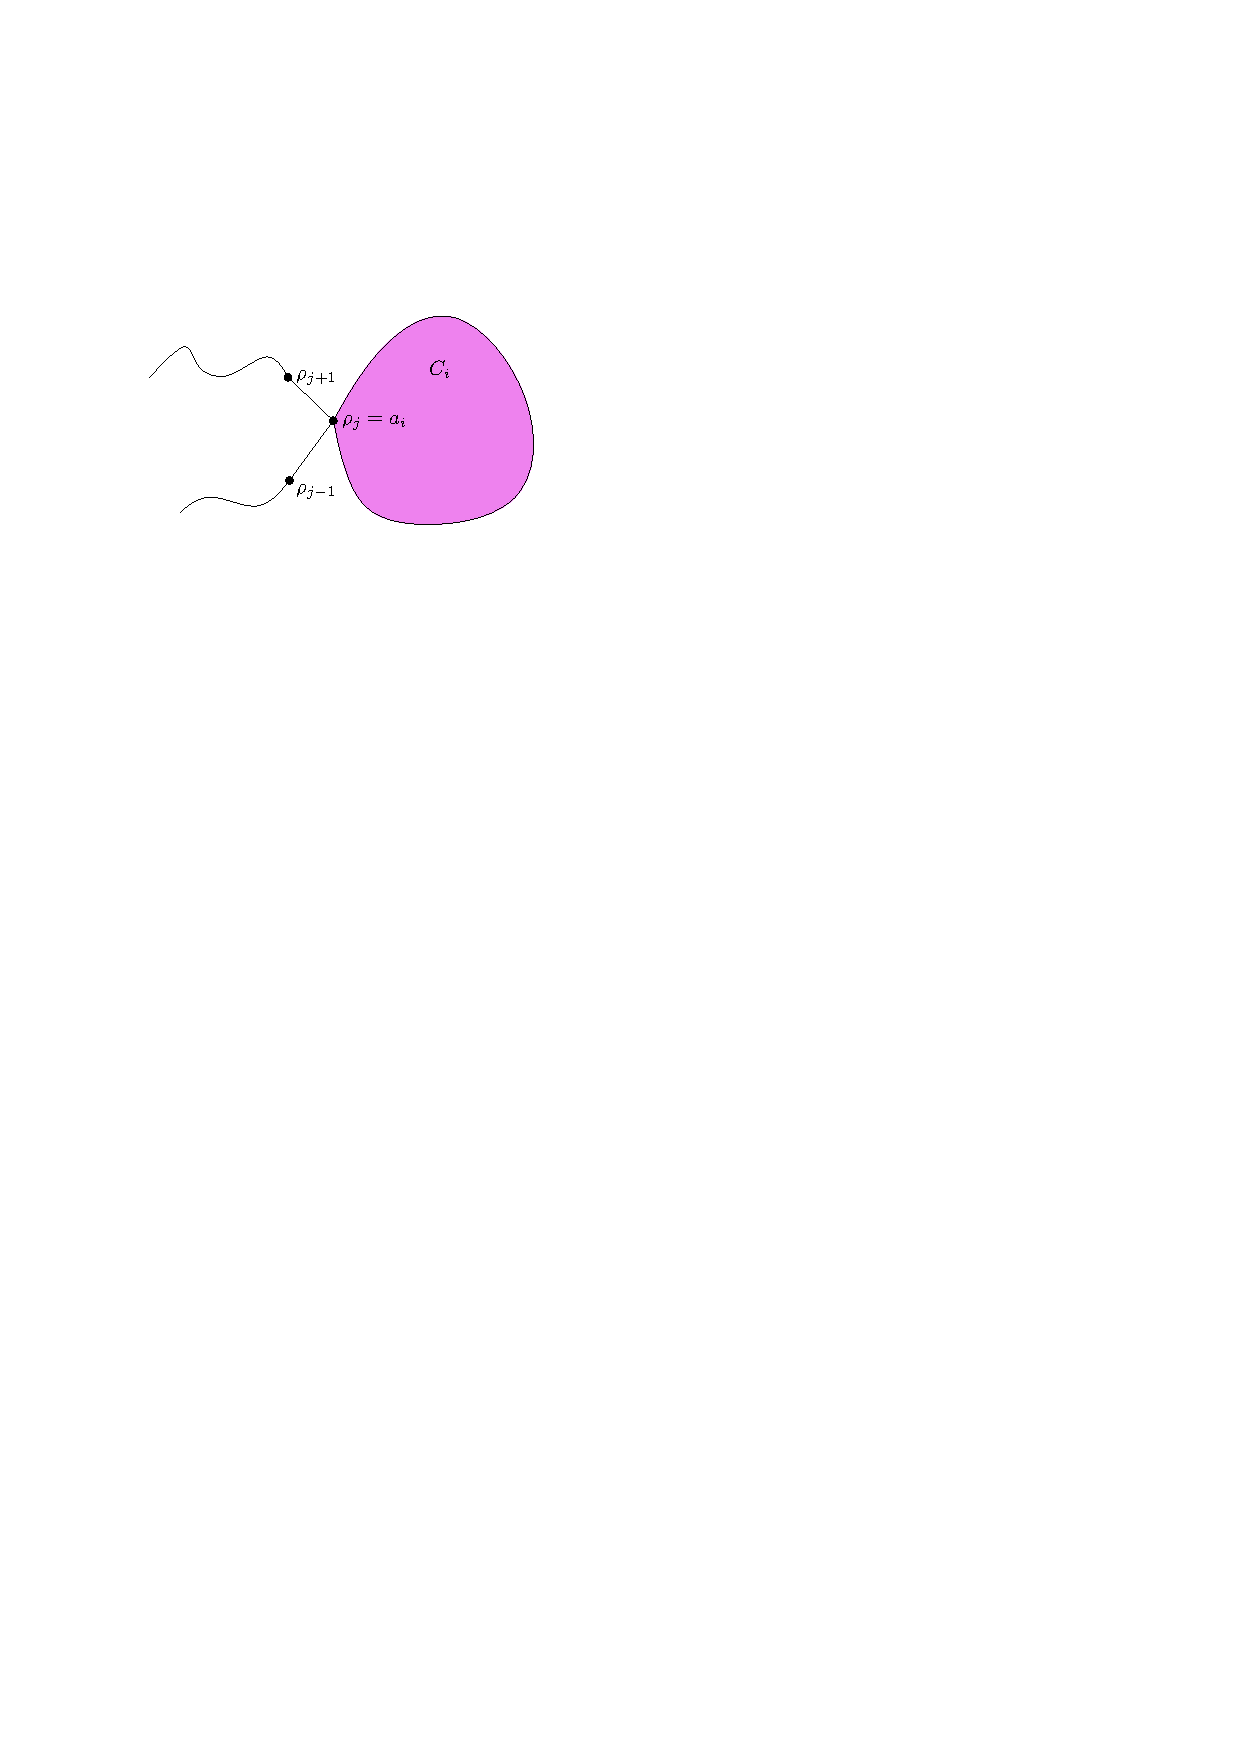
\includegraphics{img/right-of}
  \caption{The component $C_i$ is to the right of the path $R=(\rho_1,\ldots,\rho_t)$.}
   \label{figure:right-of}
\end{figure}

We want to construct a path $R$ (possibly containing Steiner vertices) that connects the attachment corners of $G$ in the given order, i.e., if $i < j$, then $a_i$ is visited before $a_j$ by $R$.
We want to construct $R$ in such a way that each component $C_i$ of $G$ lies to the right of~$R$.
Moreover, we want that $|R| = O(\sum_{j=1}^{n-1} \sigma_G(a_j, a_{j+1}))$.
We construct such a path incrementally, starting with the trivial path that contains only $a_1$.

Recall that  for any given $\varepsilon >0$, $\partial_\varepsilon G^*$ denotes the $\varepsilon$-fattening of $G^*$ (see Section~\ref{section:Preliminaries}). 
Let $\mu>0$ be a small constant to be specified later.
Initially, let $\varepsilon = 2\mu$ and let $\delta = \mu/2$. Let $\lambda < \mu/2^{r+1}$ be a constant sufficiently small so that $\partial_\lambda C_i \cap \partial_\lambda C_j = \emptyset$ for each $i,j\in\{1,\ldots,r\}$.
Throughout, $\lambda$ remains constant while $\varepsilon$ and $\delta$ are redefined on each round. However, as an invariant we maintain $\lambda < \delta < \varepsilon$.

For each $1\leq i\leq r$, let $w_i$ be the $\varepsilon$-copy of  $a_i$.
Split $\partial_\varepsilon G^*$ at $w_1$, i.e., $\partial_\varepsilon G^*$ is a path with both endpoints equal to $w_1$.
By choosing $\varepsilon$ sufficiently small, we guarantee that $\partial_\varepsilon G^*$ is simple, i.e., $\partial_\varepsilon G^*$ is isomorphic to $\varphi$.

We say that two points in the plane are \emph{$R$-visible} if the open segment joining them does not intersect $R$.
Let $\tau >0$. For each $1\leq i\leq r$ such that $a_i$ is not an interior point of $R$, consider the set of points $N_i\subset \partial_\varepsilon G^*$ that are at distance at most $\tau$ from $w_i$. 
Let $\Delta_i$ be the convex hull of $\ch{N_i\cup \{a_i\}}$, i.e., $\Delta_i$ is a ``cone'' with apex at $a_i$; see Figure~\ref{fig:Neighborhood}. (We deliberately misuse the word ``cone'' here because the ``cones'' $\Delta_1,\ldots,\Delta_r$ in this section play the same roles as the cones $\Delta_1,\ldots,\Delta_n$ in Section~\ref{section:Trivial components}.)

Throughout, we maintain also the \emph{escape invariant} which states that (1) $R$ intersects neither $\partial_\varepsilon G^*$ nor its unbounded face; (2) for each $a_i\notin V(R)$, $R$ intersects neither the simple polygon bounded by $\partial_\delta C_i$ nor the cone $\Delta_i$; and (3) $\Delta_i\cap \Delta_j = \emptyset$, for each $i,j\in\{1,\ldots,r\}$.

In particular, the escape invariant implies that every point in $N_i$ is $R$-visible from $a_i$ (including $w_i$).
Note that the escape invariant holds at the beginning, provided that the initial choice of $\tau$ is sufficiently small.

\begin{figure}[tb]
\centering
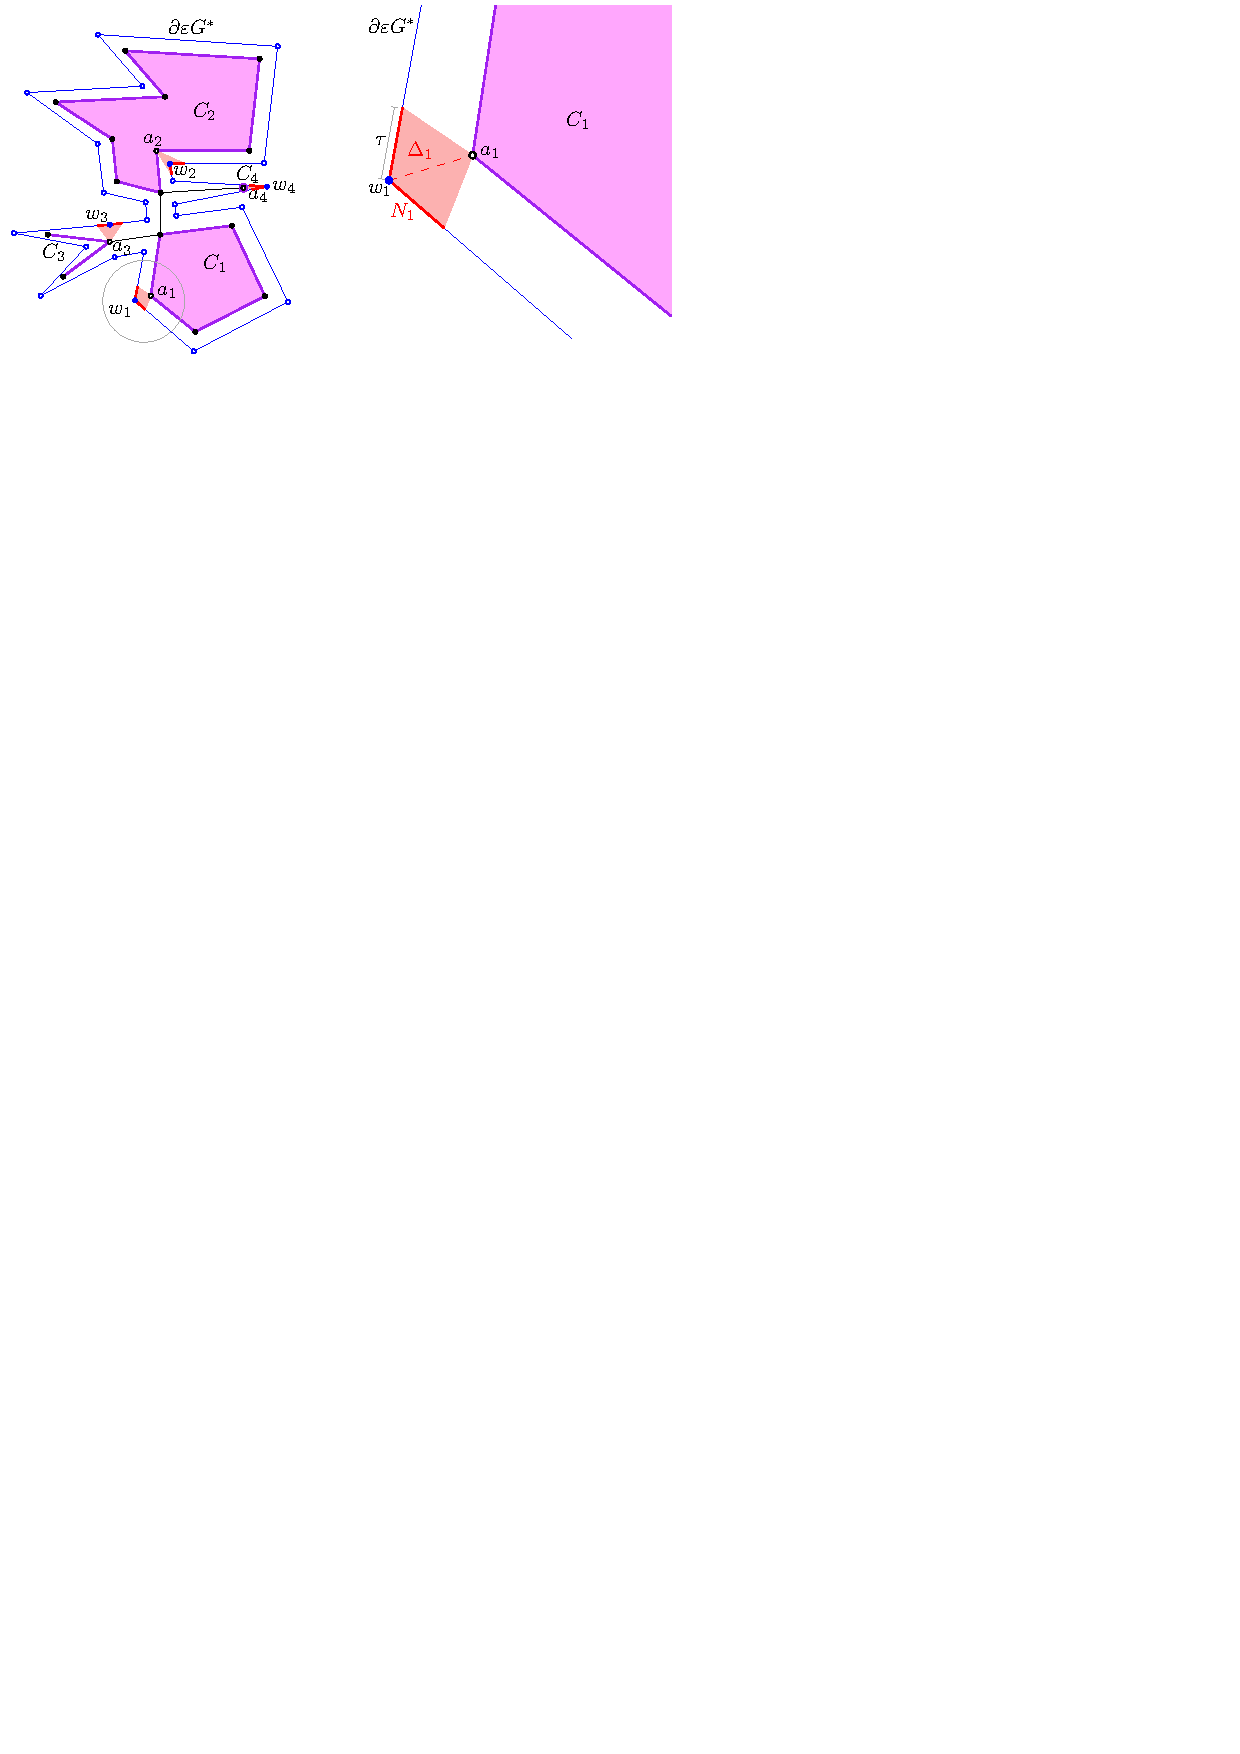
\includegraphics{img/Neighborhood.pdf}
%[width=1\textwidth]
\caption{The $\epsilon$-fattening of $G^*$ and the ``cones'' $\Delta_1,\ldots,\Delta_r$.}
\label{fig:Neighborhood}
\end{figure}

Assume that we have constructed a path $R$ that connects $a_1$ with $a_j$
for some $j\in\{1,\ldots,r-1\}$.  Moreover, assume that the escape
invariant holds.  To extend $R$, we create a new path that connects
$a_j$ with $a_{j+1}$ without crossing $R$ while maintaining the escape
invariant.  Recall that we consider $\partial_\varepsilon G_i^*$ to be
a path with both endpoints on~$w_1$.


If $j>1$, then we need to be careful in the neighbourhood of $a_j$ as we want $R$ to have $C_j$ to its right. 
If the path $R$ together with the edge $a_j w_j$ leaves $C_j$ to its right, then walk from $a_j$ to $w_j$ in straight line.
Because the escape invariant holds, we know that $w_j$ is $R$-visible form $a_j$ and hence, this edge does not cross $R$.
If $R$ together with $a_j w_j$ does not leave $C_j$ to its right, then walk from $a_j$ to $\partial_\lambda C_j$ instead and traverse $\partial_\lambda C_j$ in clockwise order without crossing $R$ before moving to $w_j$ on $\partial_\varepsilon G^*$. In this way, we guarantee that $C_j$ lies to the right of the constructed path; see Figure~\ref{fig: Component to the right} for an illustration. 
Because $\lambda < \delta < \varepsilon$ and since $a_i\in V(R)$, the escape invariant is preserved.

\begin{figure}[tb]
\centering
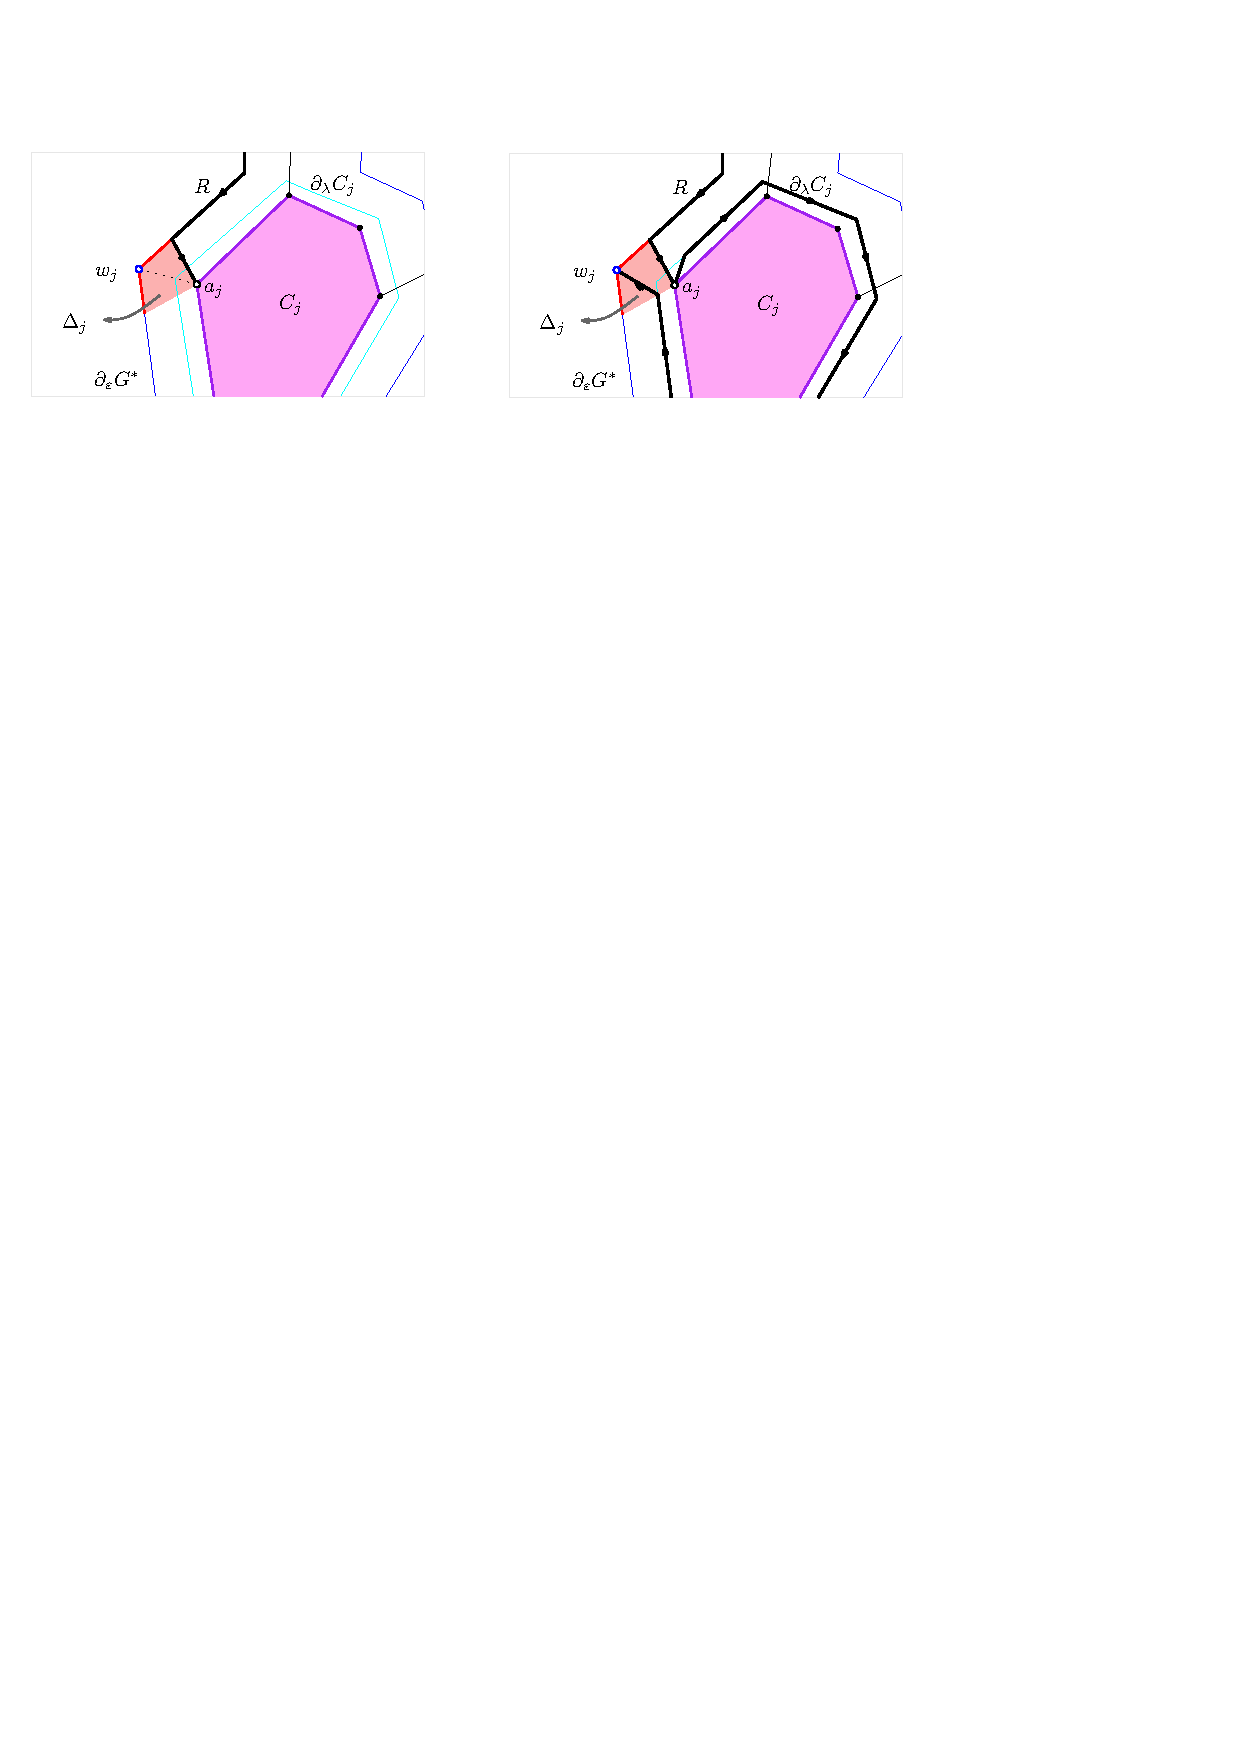
\includegraphics[width=1\textwidth]{img/ComponentToTheRight.pdf}
\caption{When extending $R$ from $a_j$ to $a_{j+1}$ we have to take care to
    keep $C_j$ to the right of $R$.}
\label{fig: Component to the right}
\end{figure}

After reaching $w_j$, we follow $\partial_\varepsilon G^*$ along the unique path that connects $w_j$ with $w_{j+1}$. 
However, whenever we reach an endpoint of $N_i$ for some $1\leq i\leq r$ such that $a_i\notin V(R)$, we take a detour to the other endpoint of $N_i$ while avoiding its interior so that the points in the interior of $N_i$ remain $R$-visible from $a_i$; see Figure~\ref{fig:Skip Component}. Formally, we walk from the reached endpoint of $N_i$ to $\partial_\delta C_i\setminus \Delta_i$ along the boundary of $\Delta_i$. Then, we traverse the path $\partial_\delta C_i\setminus \Delta_i$ before moving to the other endpoint of $N_i$ from the endpoint of $\partial_\delta C_i \setminus \Delta_i$. In this way, we avoid crossing the cone $\Delta_i$. 
Note that $R$ does not intersect the interior of the simple polygon bounded by $\partial_\delta C_i$ nor the interior of $\Delta_i$.
Moreover, $R$ never goes out of the simple polygon bounded by $\partial_\varepsilon G^*$.

\begin{figure}[tb]
\centering
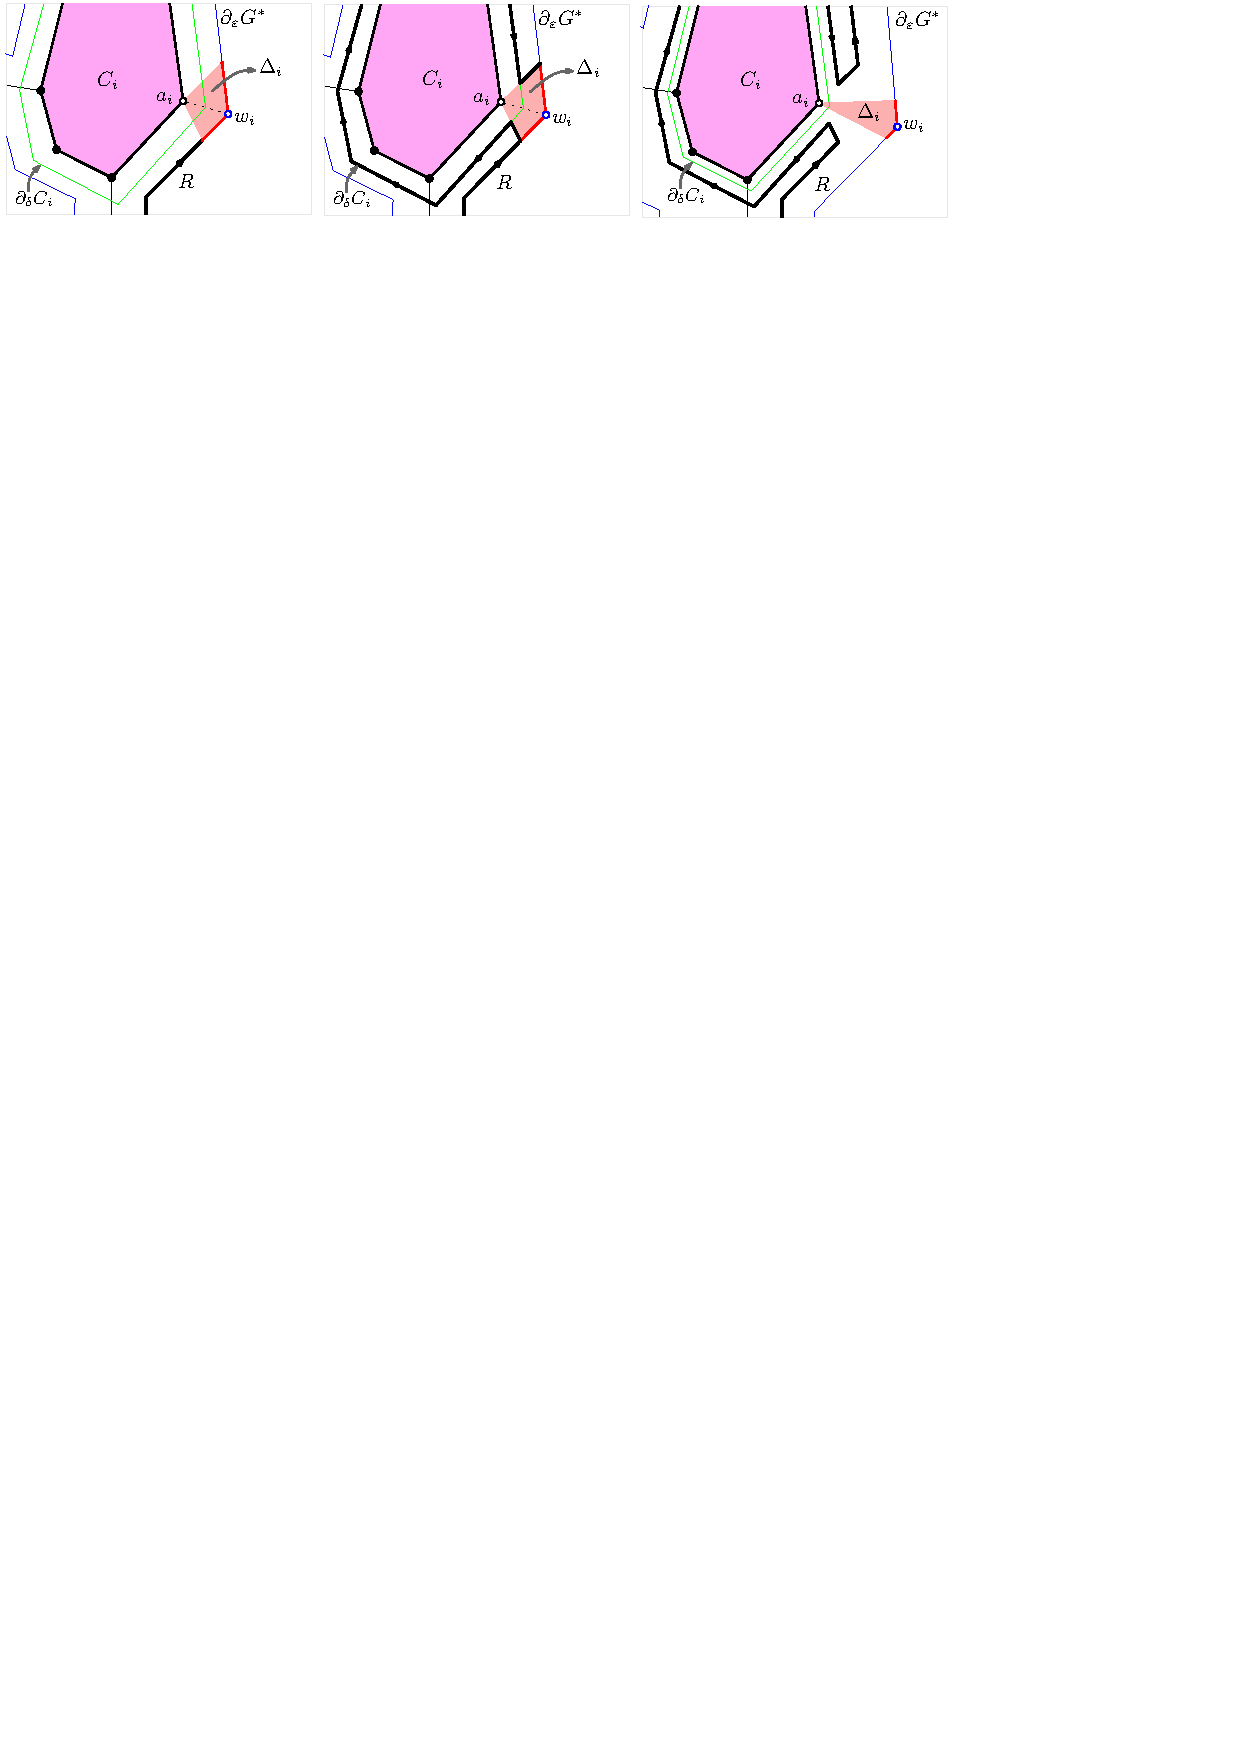
\includegraphics[width=.98\textwidth]{img/SkipComponent.pdf}
\caption{\small }
\label{fig:Skip Component}
\end{figure}

Once we go around $C_i$, we are back on $\partial_\varepsilon G^*$ on the other endpoint of $N_i$. In this way, we continue going towards~$w_{j+1}$ along $\partial_\varepsilon G^*$ until reaching an endpoint of $N_{j+1}$.
Once we reach an endpoint of $N_{j+1}$, we move directly from this endpoint to $a_{j+1}$.

Because $\partial_\varepsilon G^*$ is isomorphic to $\varphi$, the constructed $a_j$-$a_{j+1}$-path has length at most $|\varphi(a_j, a_{j+1})|$ plus the length of the boundaries of the components that we walked around. 
Because each avoided component has its attachment corner on the path $\varphi(a_j, a_{j+1})$ (i.e. in $A(a_j, a_{j+1})$), the length of the constructed $a_j$-$a_{j+1}$-path is 
\[ O\left(|\varphi(a_j, a_{j+1})| + \sum_{a_i\in A(a_j, a_{j+1})} |C_i|\right) = O(\sigma_G(a_j, a_{j+1})) \enspace .
\]

After reaching $a_{j+1}$, we increase $\varepsilon$ by a factor of two. Similarly, we decrease de value of $\delta$ by a factor of two. That is, after reaching $a_{j+1}$, $\varepsilon = \mu 2^{j+1}$ while $\delta = \mu/2^{j+1}$ and hence, we guarantee that $\lambda < \delta < \varepsilon$.
We can guarantee that $\partial_\varepsilon G^*$ remains simple, provided that the original choice of $\mu$ is sufficiently small. 
Finally, for each $1\leq i\leq n$, we reduce the size of the neighborhood $N_i$ by reducing $\tau$ by a factor of two and updating the cone $\Delta_i$ accordingly, i.e., we narrow the cone $\Delta_i$; see Figure~\ref{fig:Skip Component}$(c)$. 

Recall that for each $a_i\notin R$, $R$ intersected neither the interior of $\Delta_i$ nor the interior of the polygon bounded by $\partial_\delta C_i$. Moreover, $R$ never went out of $\partial_\varepsilon G^*$.
Therefore, after increasing (\emph{resp.} reducing) $\varepsilon$ (\emph{resp.} $\delta$), we preserve the escape invariant for the next round of the algorithm.
We repeat this algorithm until all attachment corners of $G$ are visited by $R$.

Figure~\ref{figure:big-example} is a schematic diagram that illustrates the preceding algorithm on a small example.  In this example, the path from $a_1$ to $a_2$ passes by $a_4$, so $R$ detours around $C_4$ in order to preserve the escape invariant at $a_4$.  After $R$ attaches to $a_2$ and $a_3$, it winds around components $C_2$ and $C_3$, respectively, in order to ensure that these components attach to the right of $R$.

\begin{figure}
   \centering{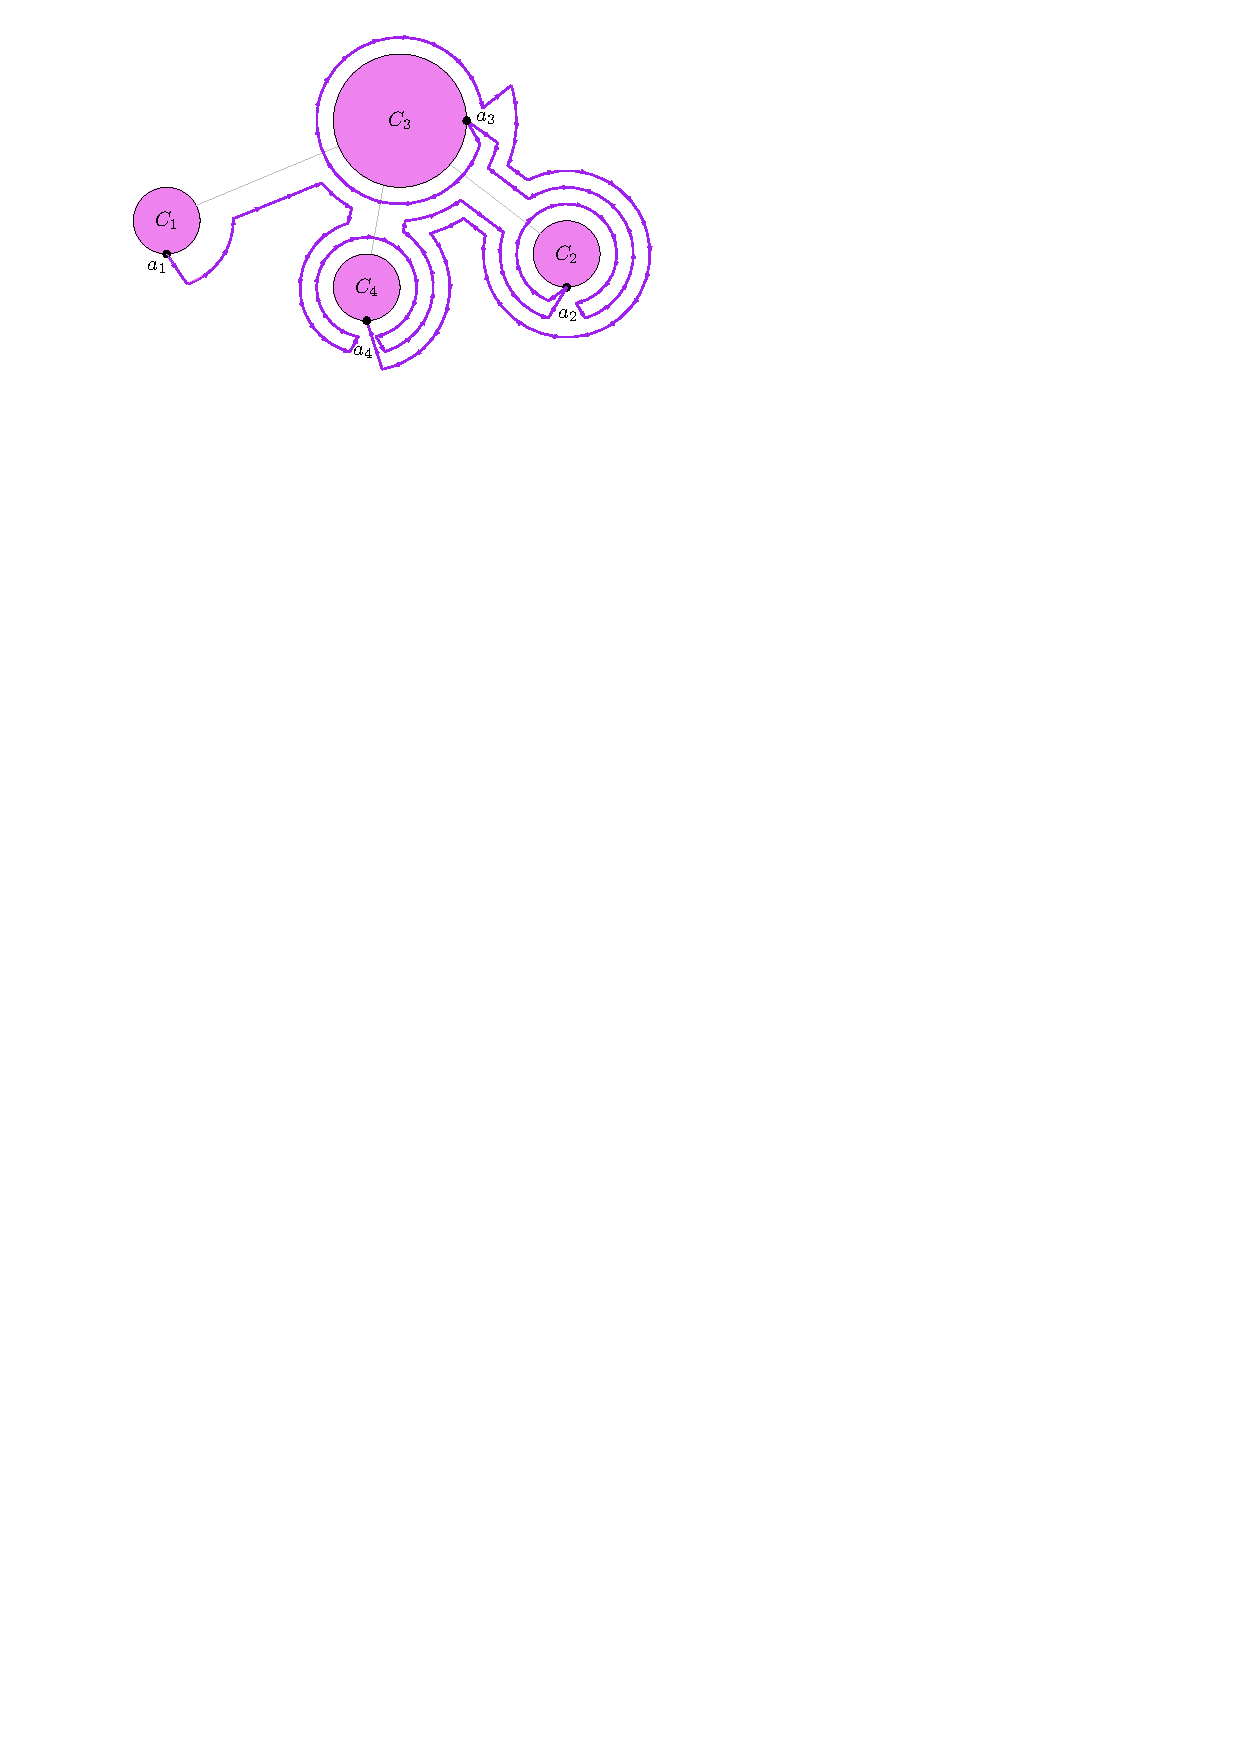
\includegraphics{img/big-example}}
   \caption{An example of the algorithm for generating a spanning path that connects $a_1,\ldots,a_4$.}
   \label{figure:big-example}
\end{figure}

\begin{lemma}\label{lemma:Path for connected augmentations}
Given an arbitrary order $a_1, \ldots, a_r$ of the attachment corners of $G$, the previous algorithm computes a path $R$ connecting all attachment corners of $G$ in the given order such that $R\cup G$ is plane, $|R| = O(\sum_{j=1}^{n-1} \sigma_G(a_j, a_{j+1}))$, and for each $i\in\{1,\ldots,r\}$, $C_i$ lies to the right of $R$ when oriented from $a_1$ to $a_r$.
\end{lemma}
\begin{proof}
By construction, the attachment corners are visited by $R$ in the given order. For each component $C_i$, $a_i$ is the only vertex of $C_i$ visited by $R$. Moreover, the construction guarantees that $C_i$ lies to the right of $R$ when oriented from $a_1$ to $a_r$.

To prove that $R$ is plane, recall that in each round we extend $R$ by constructing  a path $\gamma_j$ that connects $a_j$ with $a_{j+1}$. We claim that at this point, no edge of $\gamma_j$ crosses the portion of $R$ constructed so far.
Indeed, because the value of $\varepsilon$ (\emph{resp.} $\delta$) increases (\emph{resp.} decreases) in each round, the edges of $\gamma_j$ that lie on the boundaries of some $\partial_\delta C_i$ or on $\partial_\varepsilon G^*$ cannot cross $R$ by the escape invariant.
Moreover, this invariant states that for each $a_i\notin R$, $R$ does not intersect~$\Delta_i$.
Because each cone $\Delta_i$ is narrowed in each round, the edges of $\gamma_j$ that lie on the boundary of this cone cannot cross $R$. Finally, because $\lambda < \delta$, the edges of $\gamma_j$ that lie on $\partial_\lambda C_j$ do not cross $R$. Therefore, we conclude that by concatenating $\gamma_j$ and $R$, we obtain a plane path.

Because the length of $\gamma_j$ is $O(\sigma_G(a_j, a_{j+1}))$, the total length of $R$ after connecting every attachment corner is given by $|R| = O(\sum_{j=1}^{n-1} \sigma_G(a_j, a_{j+1}))$.
\end{proof}

\subsection{Compatible drawings of planar graphs}
Let $\mathcal G$ be a planar graph with $n$ vertices and $r$ connected components.
Let $G_1, \ldots, G_k$ be $k$ plane isomorphic drawings of $\mathcal G$. 
For now, we will assume that, in these drawings, every component of $\mathcal G$ has at least one vertex incident on the outer face.  At then of this section, we will show how to remove this restriction.
We show how to construct a compatible augmentation of $\mathcal G$ of size $O(nr^{1-1/k})$.

Let $\mathcal C_1, \ldots, \mathcal C_r$ be the connected components
of $\mathcal G$.  Because the drawings $G_1,\ldots,G_k$, all the plane
drawings of $\mathcal G$ that we consider are isomorphic, we can select
one attachment corner from each component in the drawing $G_1$, and this
attachment corner also appears in each of the drawings $G_2,\ldots,G_k$.
Thus, for each $j\in\{1,\ldots,r\}$, we can choose an attachment corner
$a_j$ of $\partial C_j$ such that $a_j$ is adjacent to the outer face
of $C_j$.

For each $1\leq j\leq r$, let $G_j^*$ be a connected augmentation of $G_j$, as defined in Section~\ref{section: connected augmentations}.
For each $i\in\{1,\ldots,k\}$ and for each $j\in\{1,\ldots,r\}$, let $\rank_i(j) = \sigma_{G_i}(a_1, a_j)$.
For each $j\in\{1,\ldots,r\}$, we define a point $x_j\in \mathbb{R}^k$ that correspond to the component $C_j$ such that 
$x_j = (\rank_1(a_j), \rank_2(a_j), \ldots, \rank_k(a_j))$. Let $X = \{x_1, \ldots, x_r\}\subset\R^k$ denote the resulting set of points
and observe that Lemma~\ref{lemma:Contained in integer grid} implies that $X$ is contained in an integer grid of side length $4n$.

Let $P$ be the shortest Euclidean Hamiltonian path of $X$, i.e., the shortest path that visits every point of $X$.
Because $X$ is contained in the $k$-dimensional integer grid of side-length $4n$ and $|X| = r$, the maximum (Euclidean) length of the path $P$ is
$O(nr^{1-1/k})$~\cite{steele.snyder:worst}. 
The order of the points in $P$ induces an order on the components of $\mathcal G$ and hence, an order on the attachment corners of each $G_i$. 

\begin{theorem}\label{theorem:main}
For each $1\leq i\leq k$, we can construct a path $R_i$ of length $O(nr^{1-1/k})$ that connects every component of $G_i$ such that $G_i\cup R_i$ is plane. Moreover, for each $1\leq i<j\leq k$, $G_i\cup R_i$ is isomorphic to $G_j\cup R_j$.
\end{theorem}
\begin{proof}
For each $G_i$, we use Lemma~\ref{lemma:Path for connected augmentations} to construct a plane path $R_i$ that connects the attachment corners of $G_i$ in the order induced by $P$.
Assume that $(a_1, \ldots, a_r)$ is the order of the attachment corners of $G_i$ induced by $P$.
Lemma~\ref{lemma:Path for connected augmentations} implies that $|R_i| = O(\sum_{j=1}^{n-1} \sigma_{G_i}(a_j, a_{j+1}))$.

Because $\sigma_{G_i}(a_j, a_{j+1}) = |\sigma_{G_i}(a_1, a_{j+1}) - \sigma_{G_i}(a_1, a_j)|$ by Lemma~\ref{lemma:Contained in integer grid} and from the fact that $\rank_i(j) = \sigma_{G_i}(a_1, a_j)$, we get that  $\sigma_{G_i}(a_j, a_{j+1}) = |\rank_i(j+1) - \rank_i(j)|$.
Therefore, $|R_i|  = O\left(\sum_{j=1}^{n-1} |\rank_i(j+1) - \rank_i(j)|\right)$.

Let $d_j$ denote the distance between $x_j$ and $x_{j+1}$ in $P$. 
Because $|\rank_i(j+1) - \rank_i(j)|$ represents the difference in the $i$-th coordinates of $x_j$ and $x_{j+1}$, by the triangle inequality we infer that $|\rank_i(j+1) - \rank_i(j)| \leq  d_j$ . 
Therefore, the path contained in $R_i$ has length $O\left(\sum_{j=1}^{n-1} |\rank_i(j+1) - \rank_i(j)|\right) = O(\sum_{j=1}^{n-1} d_j)$. 
Because $\sum_{j=1}^{n-1} d_j = |P| = O(nr^{1-1/k})$, the length $R_i$ is $O(nr^{1-1/k})$.

Since each $R_i$ visits each component only at its attachment corner and from the fact that $R_i$ leaves every component to the right when oriented from $a_1$ to $a_r$, we conclude that $G_i\cup R_i$ is isomorphic to $G_j\cup R_j$ for each $1\leq i<j\leq k$.
\end{proof}

\subsection{Handling interior components}

In the preceding section, we assumed that the drawings $G_1,\ldots,G_k$ of $G$ were such that every component was incident to the outer face and promised that this assumption would be removed.

To who the assumption is not necessary, observe that we can first use the preceding algorithm to connect all the components that do appear on the outer face using a polygonal path that is contained on the outer face.  The number of vertices used in this path is $O(n'r^{1-1/k})$, where $n'$ is the number of vertices on the outer face.

Next, for each interior face, $f$, that has multiple components
$C_1,\ldots,C_t$ on its boundary, we can use (a small modification of)
the preceding algorithm to connect $C_1,\ldots,C_t$ and the outer
boundary of $f$ using a path that is contained in $f$.  This path
has length $O(n_fr^{1-1/k})$.  We then repeat this step on each face.
The result is a connected augmentation of $\mathcal G$ whose total size
is $O(Nr^{1-1/k})$ where $N=O(n)$ is the total size of all faces.

\subsection{An algorithm}


We remark that Theorem~\ref{theorem:main} yields an efficient algorithm for constructing the augmentation $\mathcal{H}$, and even the embeddings $H_1,\ldots,H_k$.  The main steps involved are: 

\begin{enumerate}
  \item[Step 1:] Finding connected plane supergraphs $G_1^*,\ldots,G_k^*$
  of the drawings $G_1,\ldots,G_k$.  For each plane graph $G_i$, this
  can easily be done in $O(n\log n)$ time using, for example, a plane
  sweep algorithm that maintains the invariant that all components with
  a vertex to the left of the sweep-line are already joined by edges.
  Thus, this step takes $O(kn\log n)$ time.

  \item[Step 2:] Constructing the point set $X$ and finding the path
  $P$.  Constructing $X$ takes $O(kn)$ time, while a path $P$ of length
  $O(n^{2-1/k})$ can be obtained from an (approximate) minimum spanning
  tree of $X$.  For constant values of $k$, an approximate MST can
  be computed in $O(n\log n)$ time using the algorithm of Calahan and
  Kosaraju \cite{callahan.kosaraju:faster}.  For larger values of $k$,
  the actual minimum spanning tree can be computed in $O(kn^2)$ time.

  \item[Step 3:] Constructing each of the paths $R_1,\ldots,R_k$.
  Each of these paths is easily constructed in $O(n^{2-1/k})$ time
  once we have determined values of $\epsilon$, $\delta$, $\tau$, and
  $\lambda$ that are sufficiently small.  A more careful examination
  of our algorithm will reveal that all that is really needed is
  a value of $\varepsilon$ such that $\partial_\epsilon G_i^*$ is
  simple, for each $i\in\{1,\ldots,k\}$.  Once we have this value of
  $\varepsilon$, the values of the remaining variables can taken from
  the set $\{i\varepsilon/3r:i\in\{1,\ldots,3r\}\}$.

  It turns out that a value $\varepsilon \le cm/n$, where $m$ is the
  minimum non-zero difference between $x$ coordinates or $y$ coordinates
  in $G_1,\ldots,G_k$, and $c$ is a constant, is sufficiently small.
  Thus, a suitable $\varepsilon$ can be computed in $O(kn\log n)$ time
  by sorting.
\end{enumerate}

This yields the following algorithmic result about connected augmentations:

\begin{theorem}
  An augmentation satisfying the conditions of Theorem~\ref{theorem:main}
  can be computed in $O(kn^2)$ time for any value of $k$.  If $k$ is
  constant, then the augmentation can be computed in $O(nr^{1-1/k})$
  time.
\end{theorem}

The latter result (for constant $k$) is optimal since, in the next section we will show that there exists inputs where every augmentation has size $\Omega(n^{1-1/k})$.


\section{Lower Bounds}\label{section:Lower bound}

Our lower bounds are based on the following lemma. In words, this lemma says that we can find $k$ permutations of $\{1,\ldots,r\}$ such that, for half the indices $i\in\{1,\ldots,r\}$, and every $j\in\{1,\ldots,r\}\setminus\{i\}$, there is a permutation in which $i$ and $j$ are at distance $\Omega(r^{1-1/k})$.

\begin{lemma}\label{lem:permutations}
Let $t=(1/2)^{1+1/k}\cdot(r-1)^{1-1/k}$.  There exists permutations $\pi^{(1)},\ldots,\pi^{(k)}$ of $\{1,\ldots,r\}$ such that, for at least half the values of $i\in\{1,\ldots,r\}$ and for every $j\in\{1,\ldots,r\}\setminus\{i\}$, 
\begin{equation}
 \max\left\{\left|\pi^{(s)}_i-\pi^{(s)}_j\right|\colon s\in\{1,\ldots,k\} \right\}
 \ge t \enspace .
     \label{eq:perm}
\end{equation}
\end{lemma}

\begin{proof}
  This proof is an application of the probabilistic method.  Select each
  of $\pi^{(1)},\ldots,\pi^{(k)}$ independently and uniformly from among
  all $r!$ permutations of $\{1,\ldots,r\}$.  Fix a particular index $i$
  and a particular index $j$.  For a particular $s\in\{1,\ldots,k\}$, the
  probability that $|\pi^{(s)}_i-\pi^{(s)}_j|\le t$ is at most $2t/(r-1)$
  since the set
  $\{\hat \jmath\in\{1,\ldots,r\} \colon |\pi^{(s)}_i-\pi^{(s)}_{\hat
   \jmath}|\le t\}$ is a random subset of $2t$ elements drawn without
  replacement from $\{1,\ldots,r\}\setminus \{i\}$.

  Therefore, since $\pi^{(1)},\ldots,\pi^{(k)}$ are chosen independently, 
  \[
    \Pr\left\{\max\left\{\left|\pi^{(s)}_i-\pi^{(s)}_j\right|\colon s\in\{1,\ldots,k\} \right\}\le t\right\} \le (2t/(r-1))^k = \frac{1}{2(r-1)} \enspace .
  \]
  In particular, the expected number of such
  $j\in\{1,\ldots,r\}\setminus\{i\}$ is at most $1/2$ so, by Markov's
  Inequality, the probability that there exists at least one such $j$
  is at most $1/2$.  Thus, with probability at least $1/2$, the index $i$
  satisfies \eqref{eq:perm} and therefore the expected number of indices $i\in\{1,\ldots,r\}$
  that satisfy \eqref{eq:perm} is $r/2$.  We conclude that there must exist
  some permutations $\pi^{(1)},\ldots,\pi^{(k)}$ that satisfy \eqref{eq:perm}
  for at least half the indices $i\in\{1,\ldots,r\}$.
\end{proof}

Using Lemma~\ref{lem:permutations}, we can prove a lower bound that matches the upper bound obtained in our general construction.

\begin{theorem}\label{thm:lower-bound}
  For every integer $n$ and every $r\in\{1,\ldots,\lfloor n/4\rfloor\}$,
  there exists a graph $\mathcal G$ having $n$ vertices, $r$ connected
  components, and $k$ isomorphic drawings $G_1,\ldots,G_k$ such that
  any compatible augmentation of $G$ has size $\Omega(nr^{1-1/k})$.
\end{theorem}

\begin{proof}
Since the lemma only claims an asymptotic result, we may assume without
loss of generality that $r$ is even and that $2r$ divides $n$.

The graph $\mathcal G$ consists of $r$ disjoint paths,
$\mathcal{C}_1,\ldots,\mathcal{C}_r$, each of length $n/r$.  Each of the
drawings $G_1$,\ldots,$G_k$ embeds the vertices of $\mathcal G$ on the
same point and segment set. The point set consists of the vertices of
$r$ nested regular $n/r$-gons, $P_1,\ldots,P_r$, each centered at the
origin and having nearly the same size. Refer to Figure~\ref{fig:lower-bound}.a. More precisely, $P_1\subset
P_2\subset\cdots\subset P_r$ and the sizes are chosen so that any segment
joining two non-consecutive vertices of $P_i$ intersects the interior
of $P_{i-1}$.

\begin{figure}
  \begin{center}
  \begin{tabular}{cc}
    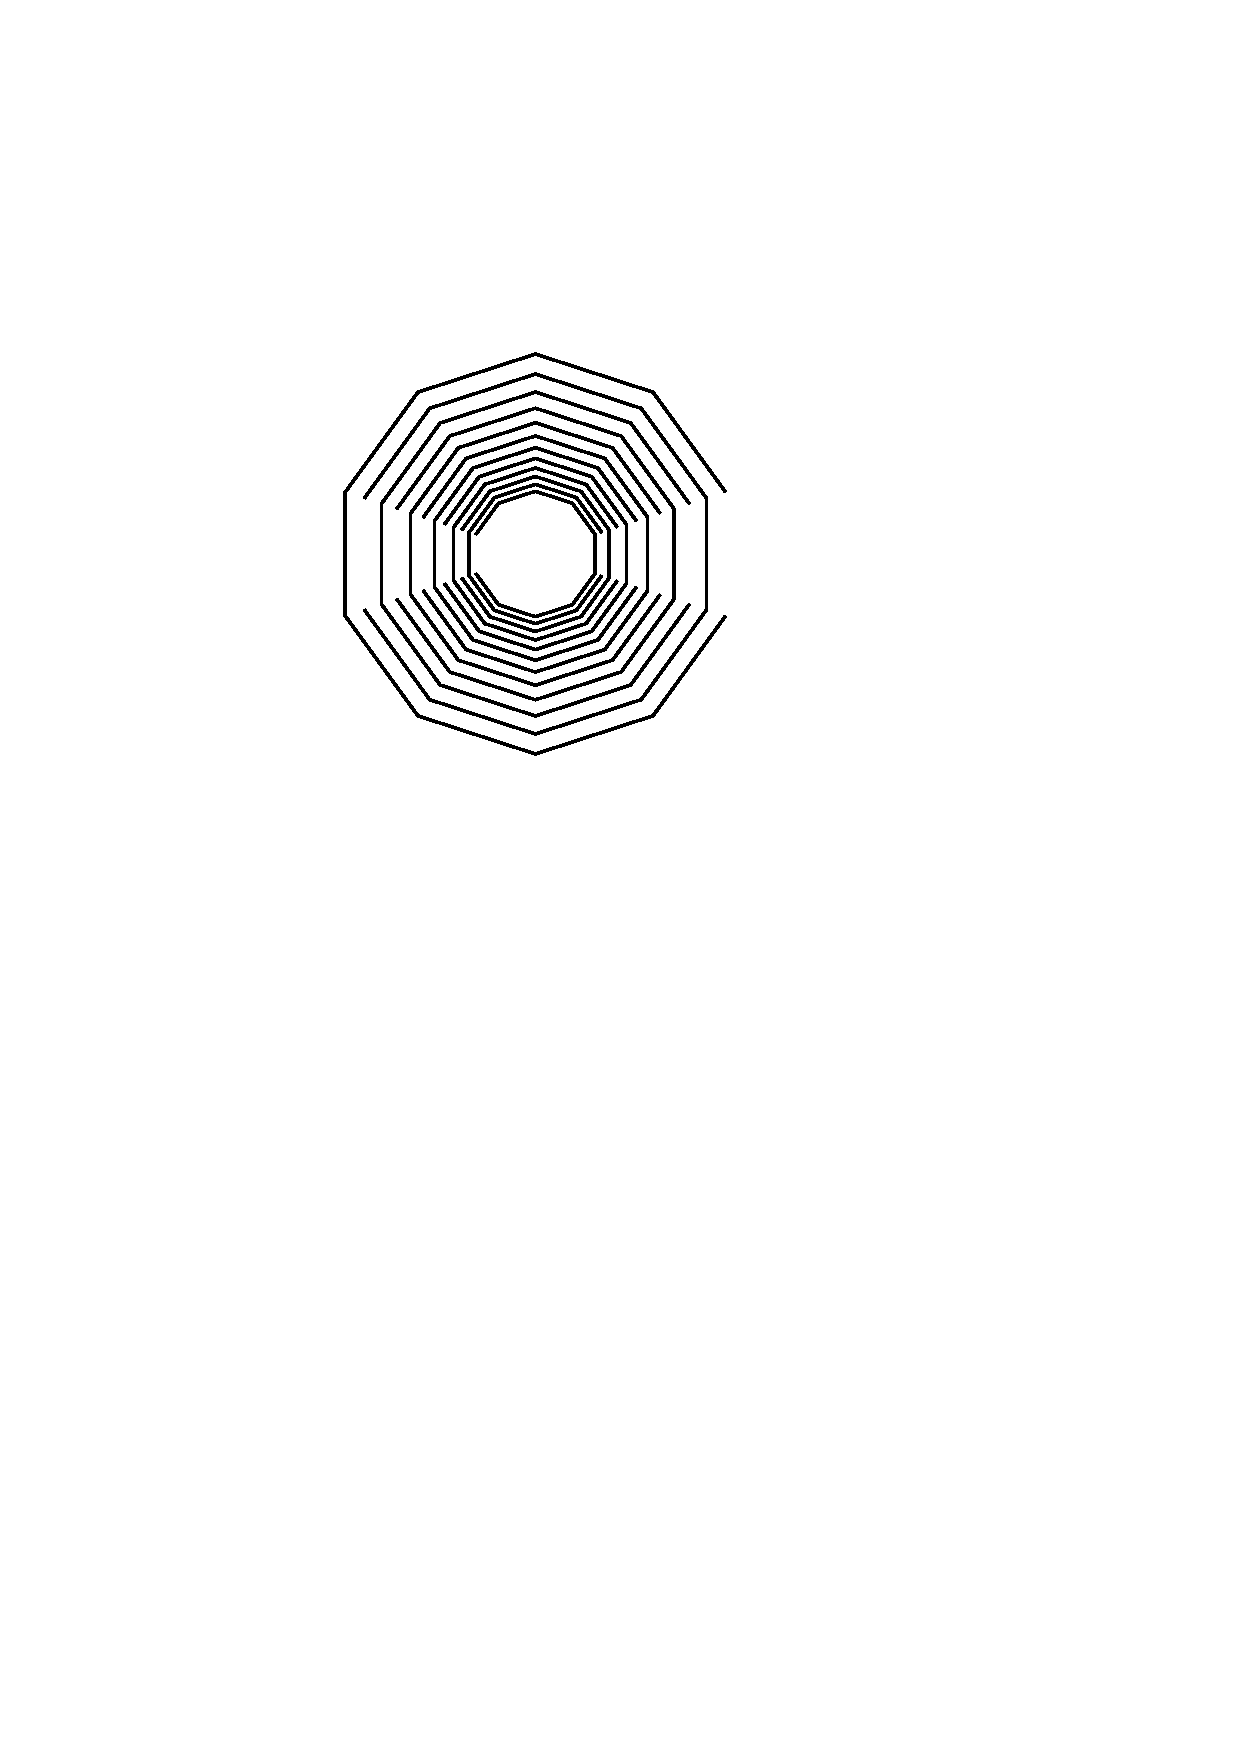
\includegraphics{img/lower-bound-1} &
    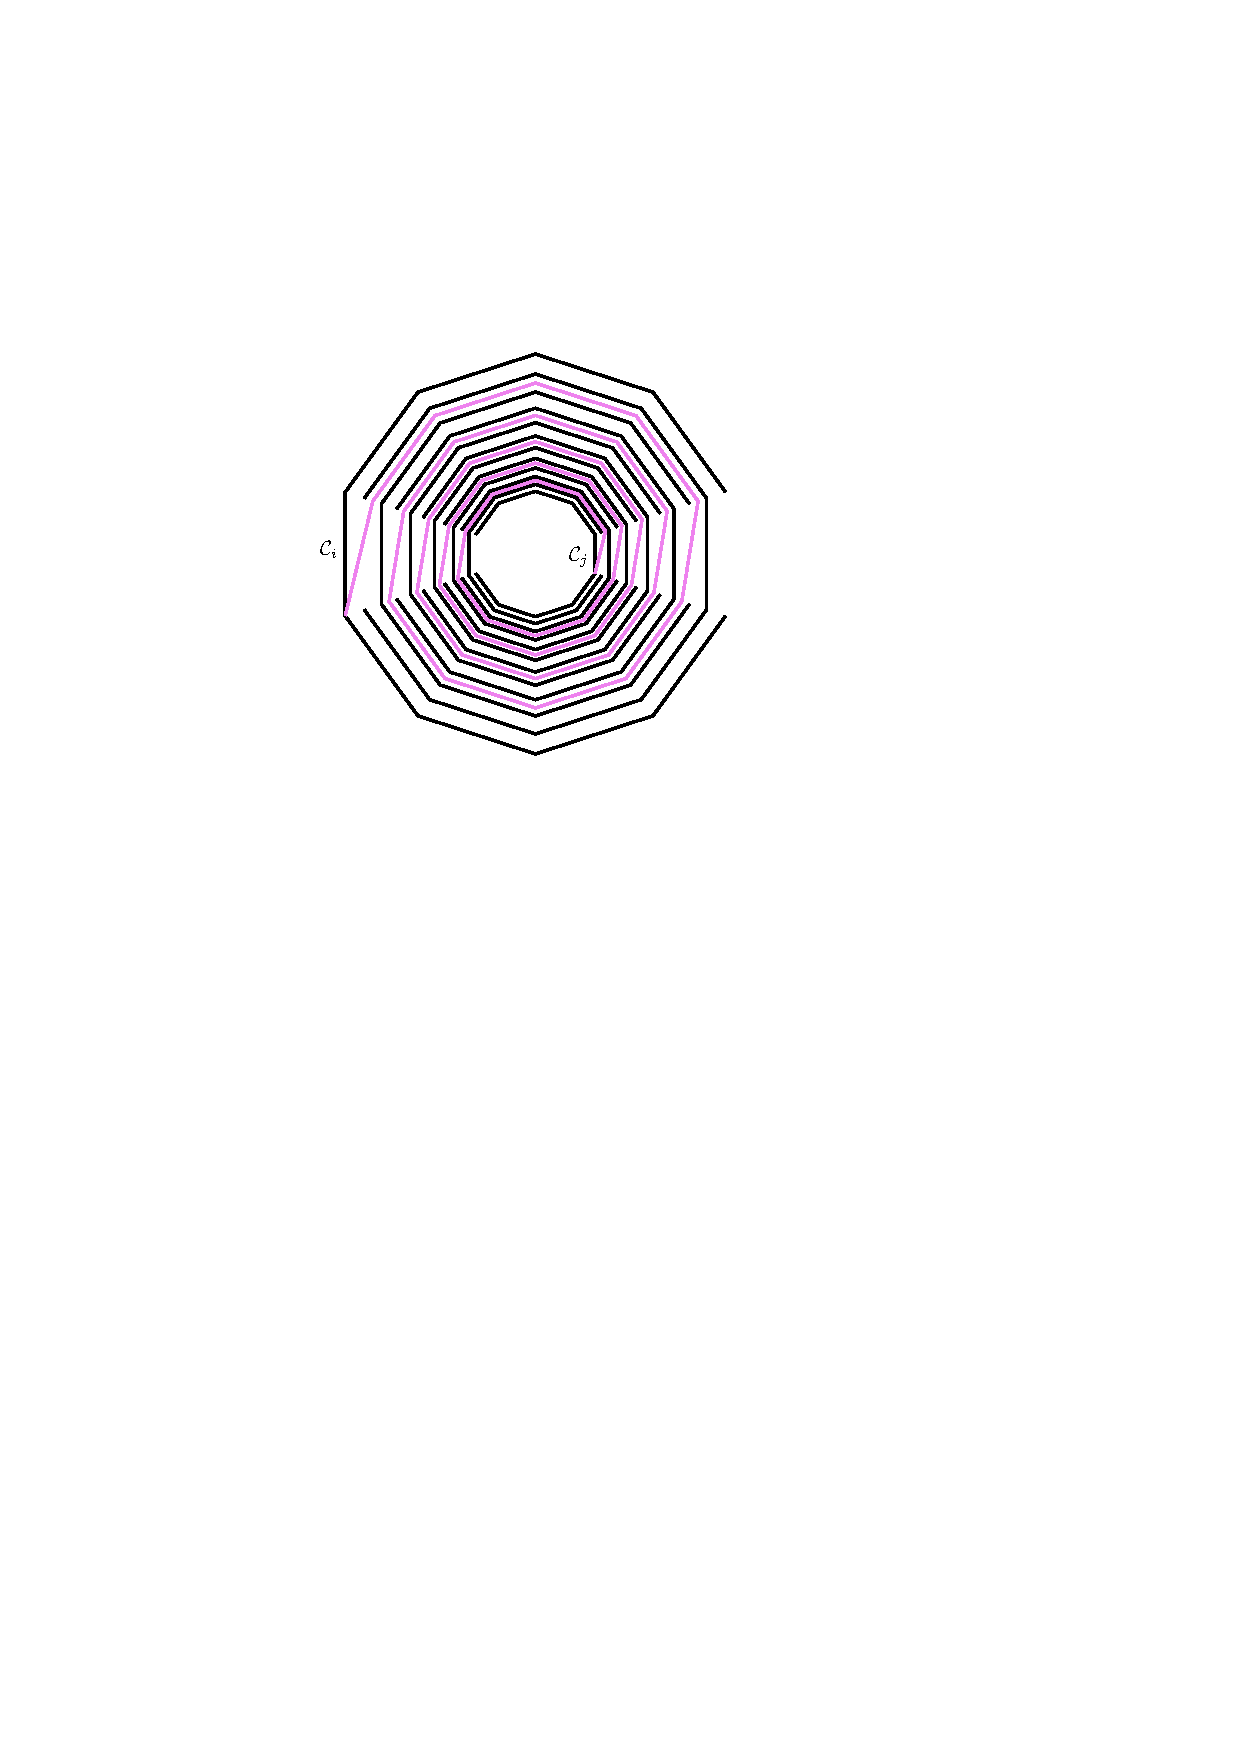
\includegraphics{img/lower-bound-2} \\
    (a) & (b)
  \end{tabular}
  \end{center}
  \caption{In the lower bound of Theorem~\ref{thm:lower-bound}, (a)~all
    drawings use the same set of points for vertices and segments for
    edges and (b)~the drawing of a path that joins $\mathcal{C}_i$ to
    $\mathcal{C}_j$ must travel around all the paths embedded between the
    drawing of $\mathcal{C}_i$ and the drawing of $\mathcal{C}_j$.}
  \label{fig:lower-bound}
\end{figure}

The drawings $G_1,\ldots,G_k$ are obtained from the permutations
$\pi^{(1)},\ldots,\pi^{(k)}$ given by Lemma~\ref{lem:permutations}.
In the drawing $G_x$, the path $\mathcal C_i$ is embedded on the vertices
of $P_{\pi^{(x)}_i}$. If $y=\pi^{(x)}_i$ is even, the drawing uses
all the edges of $P_y$ except the left-most edge.  If $y$ is odd, the
drawing uses all the edges of $P_y$ except the right-most edge.

Now, without loss of generality, consider some edge-minimal compatible
augmentation $\mathcal H$ of $\mathcal G$.  For each component
$\mathcal{C}_i$ of $G$, let $T_i$ be any path in $\mathcal H$ that has
one endpoint on $\mathcal C_i$, one endpoint on some other component
$\mathcal{C}_j$, $j\neq i$, and no vertices of $\mathcal G$ in its
interior.

Now, for each of the $r/2$ indices $i\in\{1,\ldots,r\}$ that satisfy
\eqref{eq:perm}, the path $T_i$ joins a vertex of
$P_{\pi^{(s)}_i}$ to a vertex of $P_{\pi^{(s)}_j}$, $j\neq
i$, and $|\pi^{(s)}_i-\pi^{(s)}_i|\ge t$.  This path must
have length $\Omega(tn/r)$ since it has to ``go around'' the
paths between $P_{\pi^{(s)}_i}$ and $P_{\pi^{(s)}_j}$; see
Figure~\ref{fig:lower-bound}.b.

Thus far, we have shown that for at least $r/2$ values of
$i\in\{1,\ldots,r\}$, the component $C_i$ is the endpoint of a
path, $T_i$, of length at least $\Omega(tn/r)=\Omega(nr^{-1/k})$.
It is tempting to claim the result at this point, since
$(r/2)\cdot\Omega(nr^{-1/k})=\Omega(nr^{1-1/k})$. Unfortunately, there
is a little more work that needs to be done, since two such paths $T_i$
and $T_j$ may not be disjoint, so summing their lengths double-counts
the contribution of the shared portion.

To finish up we note that, since the augmentation $\mathcal{H}$ is minimal,
it is a tree; $\mathcal G$ contains no cycles, so any cycle in $\mathcal H$ contains an edge not in $\mathcal G$ that could be removed.  Now, observe that if we traverse the outer face of (any planar drawing of) $\mathcal H$ then we obtain a non-simple path, $P$, that traverses each edge of $\mathcal{H}$ exactly twice. If we consider the set of maximal subpaths of $P$ with no vertex of $\mathcal G$ in their interior, we obtain a set of $r$ paths, $Q_1,\ldots,Q_{r}$ and, for every component $\mathcal C_i$ of $\mathcal G$, there is a vertex of $\mathcal C_i$ that is an endpoint of at least one such path.  Therefore, from the preceding discussion, the total length of $Q_1\ldots,Q_{r}$ is $\Omega(nr^{1-1/k})$.  But since each edge of $\mathcal H$ appears at most twice in these subpaths, we conclude that $\mathcal H$ has $\Omega(nr^{1-1/k})$ edges.  Since $\mathcal H$ is a tree, it has $\Omega(nr^{1-1/k})$ vertices.
\end{proof}

% \section{Summary and Conclusions}\label{section:Conclusions}
% I have nothing to write here.  Some open problems might be nice.

\bibliographystyle{plain}
\bibliography{CompatibleEmbeddings}















\end{document}  
